\documentclass[11pt,a4paper]{ujreport}
%
\usepackage{amsmath,amssymb}
\usepackage{bm}
\usepackage{graphicx}
\usepackage{ascmac}
\usepackage{float}
\usepackage{listings,jvlisting}

%ここからソースコードの表示に関する設定
\lstset{
  basicstyle={\ttfamily},
  identifierstyle={\small},
  commentstyle={\smallitshape},
  keywordstyle={\small\bfseries},
  ndkeywordstyle={\small},
  stringstyle={\small\ttfamily},
  frame={tb},
  breaklines=true,
  columns=[l]{fullflexible},
  numbers=left,
  xrightmargin=0zw,
  xleftmargin=3zw,
  numberstyle={\scriptsize},
  stepnumber=1,
  numbersep=1zw,
  lineskip=-0.5ex
}
\newcommand{\argmax}{\mathop{\rm arg~max}\limits}
\newcommand{\argmin}{\mathop{\rm arg~min}\limits}

%
\setlength{\textheight}{40\baselineskip}
\addtolength{\textheight}{\topskip}
\setlength{\voffset}{-0.2in}
\setlength{\topmargin}{0pt}
\setlength{\headheight}{0pt}
\setlength{\headsep}{0pt}

\setlength{\textwidth}{\paperwidth}     % ひとまず紙面を本文領域に
\setlength{\oddsidemargin}{-5.4truemm}  % 左の余白を20mm(=1inch-5.4mm)に
\setlength{\evensidemargin}{-5.4truemm} % 
\addtolength{\textwidth}{-40truemm}     % 右の余白も20mmに
%
\title{脳波解析のための数学シリーズ\\
基礎編}
\author{後藤 優仁}
\date{\today}
\begin{document}
\maketitle
%
%
\tableofcontents

\newpage
\section{本書の目的}
本書は,主に脳波を用いた神経科学者を志す諸君のため,脳波解析に特化した数学の入門資料となることを望んで作成するものです.神経科学は学際的な学問領域であるため,数学的素養のある人間は勿論,高校以降数学に長らく触れていなかったもの,あるいは高校数学も物理も身を入れて学んでいない者と様々なバックグラウンドの人間が流入します.自分のような半端者と異なり医者なども多いが,彼らもやはり同様に数学的な知識については疎い事は往々にしてあります.ここで言う知識とは,単に計算が出来たり,定理を暗記している事ではありません.数学を言語的に解釈し,「つまり○○をしている」「○○に使える」といった発想が出来る事をさします.よって,この意味でも「数学くらいできるし」という考えの人も半分程度はつまずくはずです.本書の目的は,そんな諸君のため厳密な数学の議論は数学書に譲りつつ,各種数学的処理の「気持ち」の理解を提供する事にあります.本書の記述にもやもやしたものを感じる人はきっと,著者よりも数学的素養,素質のある人でしょう.申し訳ないが気になったところは適宜専門の数学書を参照されたい.\\
 電気生理的な神経科学では,脳波という特殊な時系列データを解釈するために種々の数学的手段を用います.誹りを恐れず大雑把に,大きく,大きく分類するなればこれらは三種に分けられるでしょう.一つ目は信号処理,あるいは解析学.その基礎となるのが波の分解,周波数分解であり,またこの背景には偉大なオイラーの公式があります.オイラーの公式を理解すれば,一つ目の課題はほぼクリアしたと言っても良いはずです.実際,オイラーの公式と,あとは畳み込み積分させ理解していれば脳波解析に苦労することはなくなるはずです.\\
 二つ目の分野は統計です.解析的手段によって得られた脳波の特徴量を,被験者間,タスク間,時間...様々な条件で比較し,どんな条件の時にどこにどんな違いが現れるのか,その違いは大事なものなのか...そんな議論をするために必要な学習です.これがなければ,解析して得られたデータなどたいていの場合は何の役にも立たちません.あとはまぁ,脳もなにかしらの統計的学習をしているよねという議論はよくなされているし,最近だとFree Energy Principleもそうですが脳の従っているなんらかのルールを記述するような研究をかじっていくにはどうしても必要な知識になります.やっぱベイズは大事ですよねえ,ベイズ.筆者も勉強しなければと思う次第です.\\
三つ目,簡単に言えば「その他」になります(怒られそう).つまりこれらは,必ずしも全員に必要なものではないが,脳を理解するため,特に今後の脳神経科学研究においては必要になってくるであろう数学群で,自由エネルギーやら統合情報量やらに代表されるような脳の仕組みに関する理論や,グラフ理論や力学,情報学といった新しい脳情報解析に利用される数学などです.必要になった時に学べば良いと思いますが,やはりこうした議論を何も理解していない者とそうでない者とには今後大きく差がつくであろうし,日々勉強する事は大切であるように思います.本書は解析や統計に関する記述を優先的に補充していきますが,それ以外の数学については筆者の好みで足していこうと思います.(2021.5.15)\\
  以上のような本書の目的に従い,文中では(特に後半),数式のみでなくこれらの計算を実際に手元のPCにやらせるためのソースコードも記載していく事とします.言語は迷いましたが,ひとまずはMATLABを使用し,必要を感じれば別途Pythonのソースコードを用意します.理由としては,筆者の所属ラボ含め神経科学の多くの研究室は脳波や脳磁,核磁気共鳴画像の解析にMATLABを使用している事,それによって公開されている論文のソースコードもMATLABで実装されている事,EEGLABなどのツールボックスも充実しているため使うのが楽である事,などがあります.またコードは文中にはminimumで載せますが完全版というか,資料に載せているようなplotをだすコードは同じファイル名のスクリプト( .m )ファイルで用意しておきます.気になる人はダウンロードするなりして自分の環境で実行してください.なお筆者のネイティブはPythonなので宗教戦争には巻き込まないでください.いやほんと,MATLABダサいしなんか気持ち悪いし嫌いです.ほんと.まじ嫌い.\\
\\

 さて筆者のプロフィールですが, 脳神経科学歴1年(2018年9月), 数学歴半年のペーペーです. 数学に至っては半年前は虚数が何か分からなかったし三角関数の意味も知りませんでした.\\
よって変な理解だとか知識の抜けもあると思うのでご指摘お待ちしています.\\
\\
2021/5現在は生理学研究所の博士課程です.
\\
\section{本書のカバーする内容}
本書は筆者の気が向いた時に少しずつ更新していくので, タイミングによってはほとんど書いてないと思いますが, 最終的に目指している点をここに記します.\\
\\
 基本的には脳神経科学, 特に脳波を用いる際に必要になってくる数学を全体集合として, 部分集合を小出しにだしていく感じを考えています. 補集合については更新を待つか諦めて独学をする, あるいは筆者に書くよう申請をしてください. 従って本書のカバーする内容はおおまかに分けて\\
\\
\begin{screen}
\begin{itemize}
 \item 前提となる基礎的な数学
 \item 脳波を代表とした信号を処理する信号処理数学
 \item ANOVAやt検定, 簡単な機械学習などの統計的数学
 \item その他愉快な仲間たち
\end{itemize}
\end{screen}

などといった感じになると思います. 初学者,特に実験系の人達の考える事は痛いほどに分かります.「別に数学の研究したいわけじゃないし」ですよね.しかしこれら基礎が分かっている人と分かっていない人とでは,まず先行研究に対する批判的な読み方に大きく差がつき,それが理解の差につながります.当然,転じていざ自分の研究を計画する時の綿密さにも差が付き,手を動かして解析し統計的議論をする頃には覆しえない程の差がついている事でしょう.\\
うん,言われても納得しがたいとは思いますが,実際一度研究をしてみれば分かると思います.後から「え...これ意味ないですよね」とか「この解析,信号に○○性の仮定が必要だと思うんですが今回の実験で得られるデータは○○性を満たさないのではないですか?」などと学会の発表でマサカリを投げられて致命傷を負う読者諸君が見えます.飯うまい.僕もやられたし.ほんとあれしんどいです.勉強しとけ.まじで.\\
\\
頑張って行きましょう.
\\
\\
いよいよ始まりますが,まず最初のこのbasic.pdfはこれ以降の議論を展開するために最低限身に着けておいて欲しい数学的知識,考え方です.心して確認してください.
\chapter{掛け算}
 はじめに,基礎を学ぶ上で必要になる基礎の勉強,というか確認から始めます.高校以降は文系よりだった人や,高校でも数学はやってたけど受験のための暗記数学をやっていて,正直数学についてあまり考えたことがない人向けです.以降の章でやっていく内容を読んでいく上で最低限覚えておいてほしい内容です.

\section{掛け算とは何か}
信号処理や統計といった難しい数学をこれから皆さんはやっていくわけですが,こういった数学は結局のところどこまで行っても足し算と掛け算です.脳波の解析も統計も,複雑な「数」に対応した,複雑な「足し算,掛け算」をやってあーだこーだしていく処理にすぎません.なのでまずはここで,掛け算とは何かを考えていきましょう.足し算については比較的簡単であまり違いを意識しなくても良いので,ここでは掛け算のみ触れます.\\
 伝えたいメッセージは,世の中には色々な「数」があって,対応した色々な「掛け算」がある.という事です.まずはこの事をしっかり頭に入れておけば,解析とかの勉強もさして難しくないはずです.別に全て覚える必要はないので,とにかく色々あるんだなーとだけ感じてください.
\subsection{数ってなぁに?}
まず初めに,この書において扱う数はユークリッド空間のものに限ります.非ユークリッドを持ち出してねちねちと文句は言わないでください.だから嫌われるんですよ.あぁすみません,嫌われている自覚がなかったんですね.余計な事を言ってしまって申し訳ないです.さて,先程ユークリッド空間や非ユークリッド空間といった言葉が出てきましたが, 簡単にいうとこれらは全て別の「数」として考える必要があるため, 空間と名付けられています. そもそも,「数」ってなんだろう?最初はそんなところから考えてみましょう.\\
まずは単一の数と複数の数に分けるところからいきます.\\

\subsection{単一の数スカラー}
単一の数, スカラー数です. 高校での数学を真面目に受けていた人間なら聞き覚えがえるでしょう. スカラー数とは最も簡単な数...すなわち僕達が昔から親しんできた「数」のことです!\\
簡単ですね!以上です.\\
\\
スカラー数の掛け算は僕たちが直感的にやっている
\begin{eqnarray}
\label{eq:kakezan}
3 \times 5 = 15
\end{eqnarray}

の事です.
\begin{lstlisting}[caption=式(\ref{eq:kakezan})のMATLABコード,label=sc:kakezan]
3 * 5
\end{lstlisting}

以降,ソースコードはコード(\ref{sc:kakezan})のように記載していきます.式では変数としているものも,実際に数字がないと計算できないので好きに補完しつつ実装してみてください.
\subsection{複数の数からなる積}
複数の数からなる数には色々あります.\\
\begin{itemize}
 \item ベクトル
 \item 複素数
 \item 行列
\end{itemize}

等です. これらはスカラー数の掛け算とは全く違う世界になります. 心してかかりましょう. 高校以上の数学は非常に難しいもので, 僕も全く分からずに置いて行かれましたが, どうにか理解するための最初の第一歩は, 「世の中には(スカラー)数じゃない数があるらしい」と知る事です. 僕はこれを理解するまでに無駄に長い時間を費やしてしまいました. \\
\\
 では, そもそも何故スカラー以外の数を考える必要があるのでしょうか?\\
 普通に生きていてベクトルや複素数といったものを自然の中に見る事はないでしょう(あるいは啓蒙を高めると見る事が出来るのやもしれない).\\
\\
(追記: 2019年9月現在の筆者は日常にたくさん見るようになった. 啓蒙が高まったのやもしれん.)\\
(追記: 2021年現在の筆者は上の記述が恥ずかしい.当たり前やんけ)\\
\\
 しかしスカラー数には限界があるのです. 何故なら, 基本的にスカラー数とは直線(上の点)であるからです! \\
\\
 0があって1があり, その次に2が来るのは小学2年生の数直線ですが, 小学4年生頃には「どうやら0と1の間にも小数や分数があるらしい」と知ります. 次に中学になり, 0の向こう側には同じだけの数の負の数があり, 更には√がつく数などもある事を知ります. そして少し飛びますが高校では, 数直線の右と左に終わりはなく, 無限という領域に飛んでいる事を知りますね. ここまでがスカラーの学習順序ですが, いずれも1本の直線を細かく見たり, あるいはずっと先を見ているだけです. \\
\\
 ただの直線であるスカラーでは記述できる情報が少ないため, 不都合があるから別の数を考える必要があったわけです. スカラーっぽいやつらを複数束ねてまとめた「数」を新しく定義してやれば表現できる情報量は各段に増え, 世界が広がります. \\
\\
 記述する要素が増えれば情報が増えるのは考えれば納得ですね. イメージは中学数学の1次関数のグラフとかです.縦と横,軸が増えれば情報は増えますね?
\\
\subsection{ベクトルの積}
ベクトルとは, 二次元の場合は2つ, 三次元の場合は3つの数...を束ねたものです. \\
数を複数束ねると, その間に比が生まれ,それらによって定義される長さを持った線(と基準線との角度)が生まれます. \\
 これが先述した, 増える情報量であり, スカラー数との決定的な違いです.\\
 ちなみに, この「比と角度(と長さ)」ですが, これは脳波においては位相や電位の強度といったものを考える時に必要になります. というかそのままです. よく確認しておいてください. 
\\

\begin{figure}[H]
\label{im:vector}
  \centering
  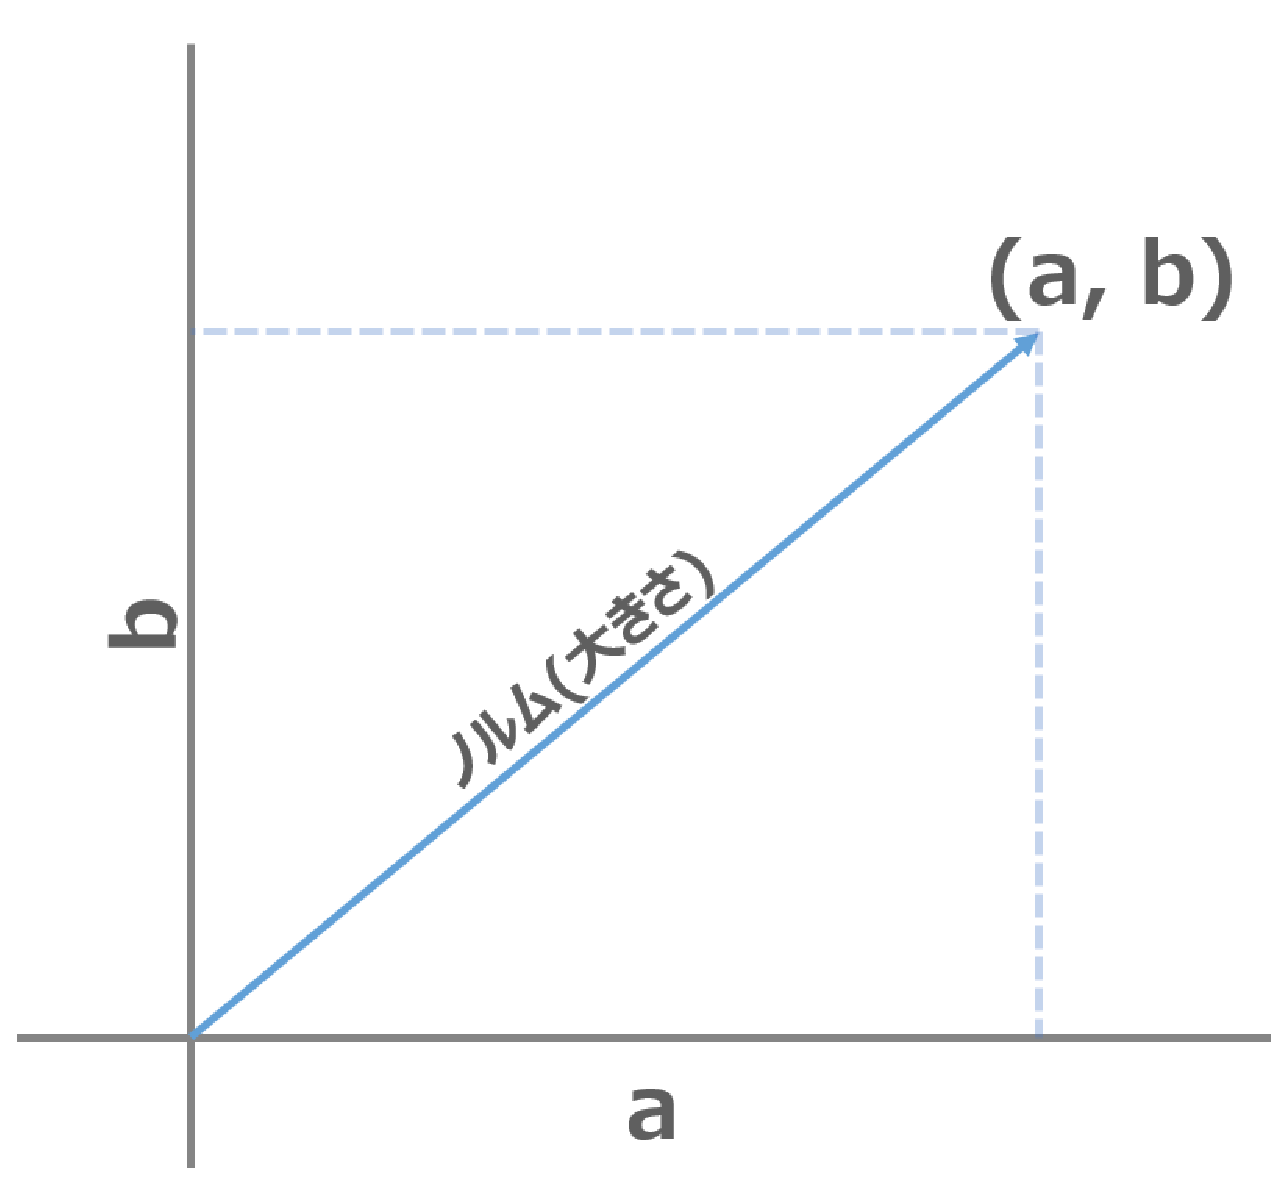
\includegraphics[width=10cm]{../figures/vector.eps}
  \caption{2次元ベクトルの例}
\end{figure}


 ベクトル同士を掛け合わせるとき, どうするでしょうか?\\
 一番素朴な形は下記の通りでしょう.\\
\begin{eqnarray}
\label{eq:veckake}
(\mathstrut x_1 , \mathstrut y_1)(\mathstrut x_2 , \mathstrut y_2 ) = (\mathstrut x_1 \mathstrut x_2 + \mathstrut y_1 \mathstrut y_2)
\end{eqnarray}

これをベクトルの内積と言います.\\
\begin{lstlisting}[caption=\ref{eq:veckake}のMATLABコード,label=sc:veckake]
x = [1 2 3]
y = [4 5 6]
dot(x,y)
\end{lstlisting}
 そして, ベクトルの内積はもう一つの算出方法がありましたね. 2つのベクトルの絶対値の積に互いになす角の cos をかけたものです. 確認してみましょう.\\

\begin{eqnarray}
\label{eq:vecdot}
\mathbf{a}\cdot \mathbf{b} = |\mathbf{a}||\mathbf{b}|cos\theta
\end{eqnarray}

まず,式(\ref{eq:vecdot})の見方ですが,太字は数学ではベクトルを表します.なので$\mathbf{a, b}$はスカラーじゃないことに注意してください.\\
 さてここからが味噌ですが,普通は上の式を見ると絶対値の積に,$cos\theta$をかけていると思うでしょうがそうではありません.考え方としては,$|\mathbf{a}|$に$|\mathbf{b}|cos\theta$をかけているという方が分かりやすくなります.あ,もちろんaとbを逆にしても大丈夫です.

では$|\mathbf{a}|$は良いとして,もう一つの方はなんだよという事が当然気になるわけですが,そこで出てくるのが射影という考え方です.

\begin{figure}[H]
\label{im:shadow}
  \centering
  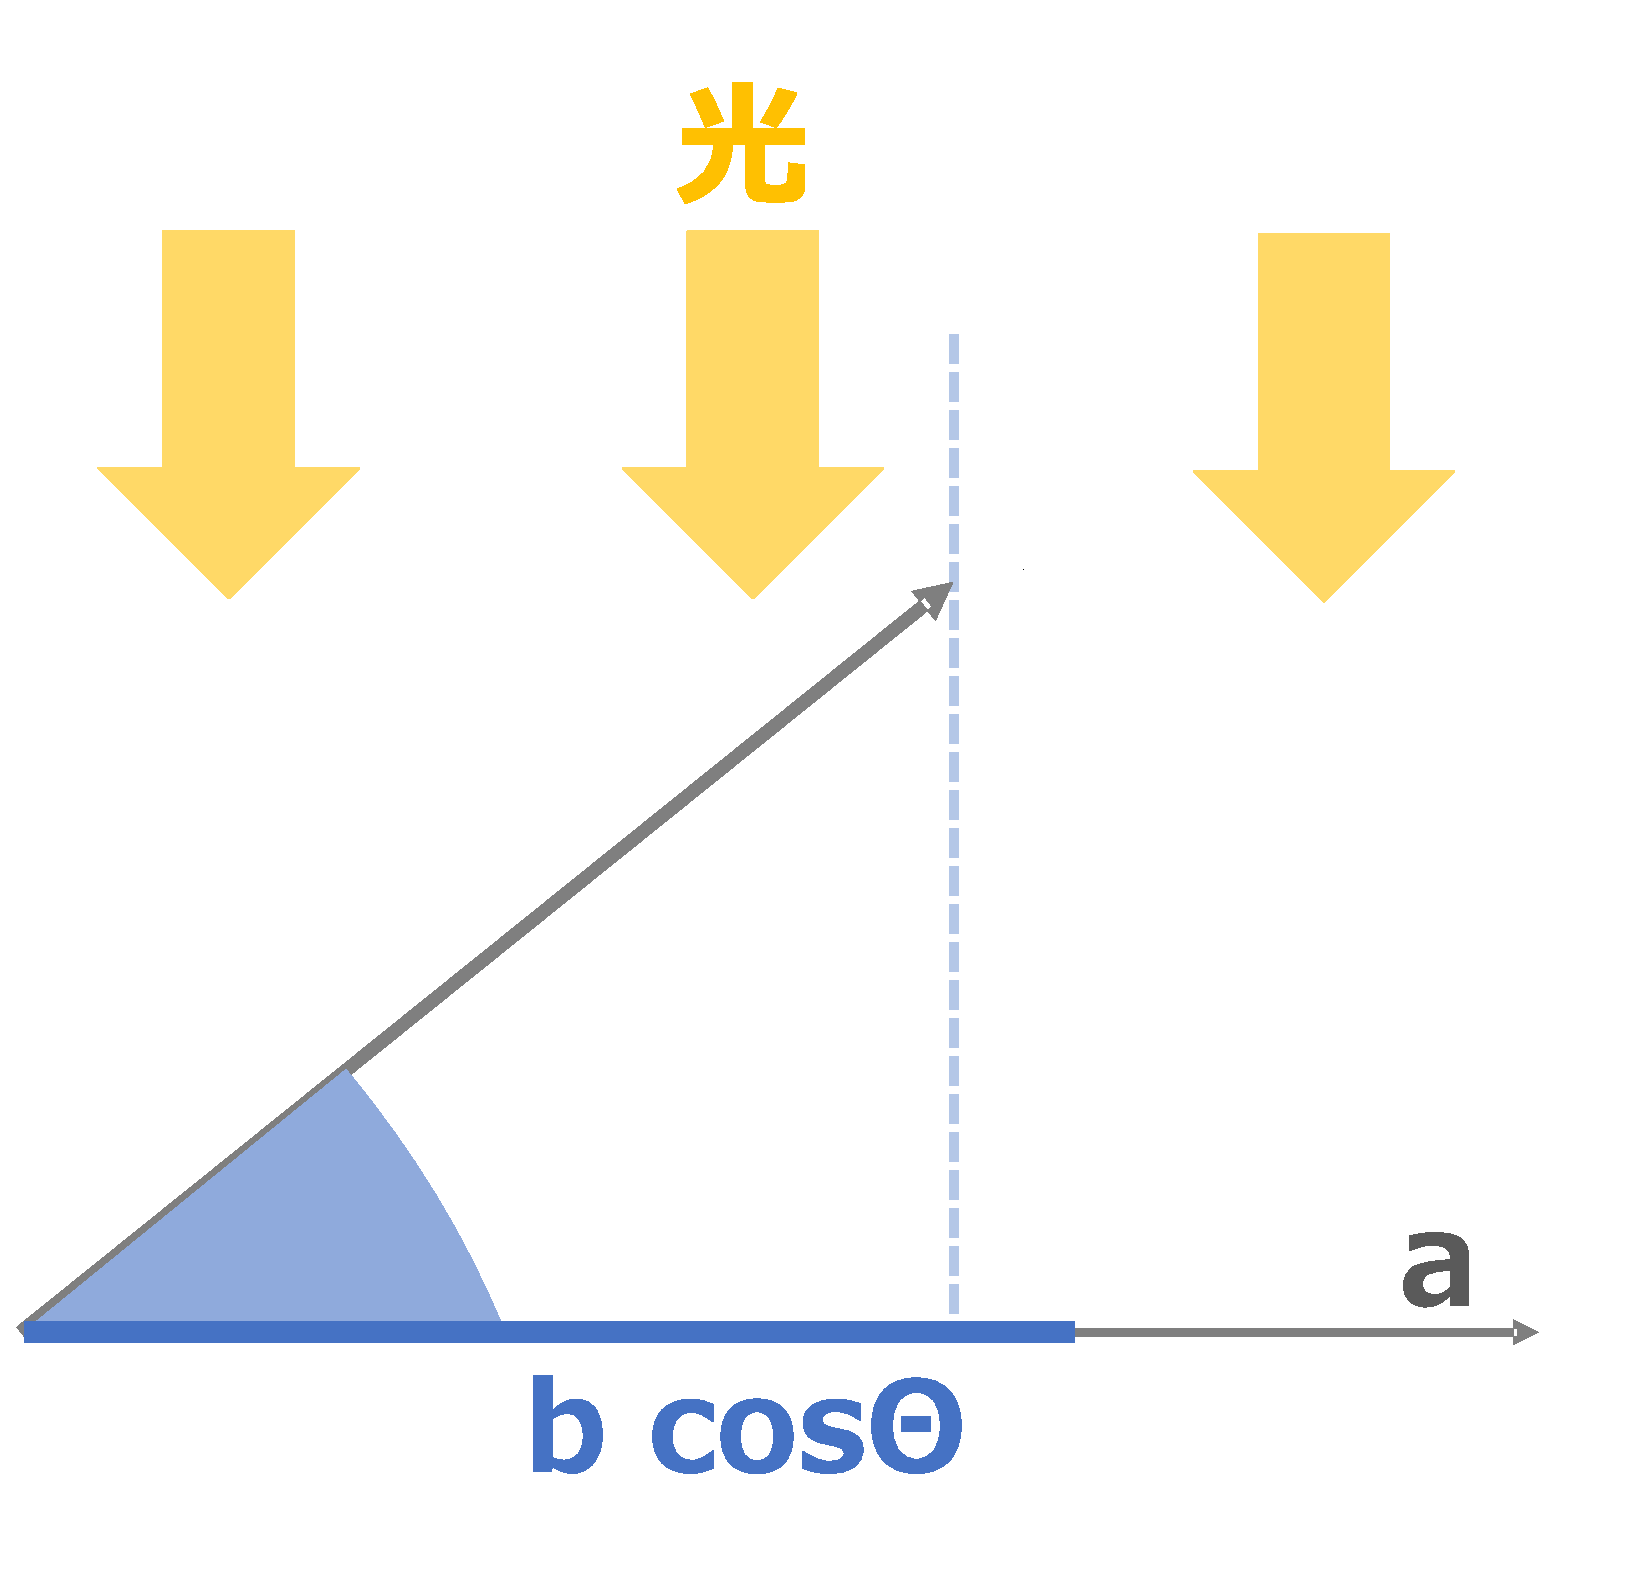
\includegraphics[width=10cm]{../figures/shadow.eps}
  \caption{ベクトルbのベクトルaに対する正射影}
\end{figure}

よくある説明は,ベクトルaに対して垂直な光によって照らされたベクトルbの影の長さ,というものです.まぁようはベクトルbの,ベクトルaの方向に対してもっている影響力とかなんかそんな感じの量です.これでベクトル同士の向きをそろえた上でかけているわけですね.\\

ここからベクトルの内積というものが何を表しているのかが分かるのですが, いったん置いといて次へ進みます.\\

\subsection{内積の意味}
内積の定義を見てきましたが, 結局のところその意味は何でしょう?\\
 先程,内積が$\mathbf{a}$と射影した$\mathbf{b}$の積である事は確認できました.ここから場合わけして考えます.まず$\mathbf{a,b}$が同じような方向を向いていた場合,$\theta$の値は小さくなり,射影されて出来る $|\mathbf{b}|cos\theta$ の値はほぼ $| \mathbf{b}|$ から変わりません.そこから角度が大きくなるにつれ値は小さくなっていき,ちょうど2つのベクトルが直行する時($\theta = \frac{\pi}{2})$に内積は0になります($\because cos\frac{\pi}{2}=0)$.\\

そしてそのまま角度を大きくしていくと,今度は射影ベクトルがベクトルaと全く重ならないようになってしまい,$cos\theta < 0$となります.つまり,二つのベクトルが直角よりなお別の向きを向いている場合,内積は負の値をとります.\\

この事をまとめると,以下のような関係が言えます.

\begin{screen}
内積の定義
\begin{align}
  \mathbf{a}\cdot\mathbf{b} &= a_1b_1 + a_2b_2\\
&= |\mathbf{a}||\mathbf{b}|cos\theta 
\end{align}

内積の取る値
\begin{align}
\mathbf{a}\cdot \mathbf{b} &> 0 \qquad \text{(ベクトルの向きが似てる時)}\\
&=0 \qquad \text{(ベクトルが直行している時)}\\
&<0 \qquad \text{(ベクトルの向きが離れている時)}
\end{align}

\end{screen}

つまり内積とは,二つのベクトルの向きの関係性を示す指標として捉える事が出来,特に0になる場合にそれらのベクトルが直行している事を示せるものです.

\subsection{ドット積}
 ベクトルの掛け算のうち, ドット積だとか点乗積と呼ばれるものがあります.ドット積とは, 同じ長さの数列の各要素を掛け合わせ, その値を足し合わせて一つの値として出力したものです.\\
\begin{align}
a = {a_1,a_2,a_3,a_4}\\
b={b_1,b_2,b_3,b_4}\\
a\cdot b = a_1b_1 + a_2b_2 + a_3b_3 + a_4b_4
\end{align}
\\
そう, つまり内積の事ですね.\\
 ドット積は実質(ユークリッド空間では)内積と同じ扱いをされます.\\
\\
 こいつは代数学・幾何学において非常に大事になる上, 畳み込みの基礎となるものです!\\
 そしてそれはつまり, フーリエ変換やウェーブレット変換(参照: analysis)の基礎になる重要な掛け算です.ベクトルの掛け算を学ぶ意味は,そもそも我々がこの先扱う事になる脳波データなどの信号は全てベクトルであるからです.ベクトルを操作する方法をしっかりと学ぶ事が必要になります.そして内積はいずれ脳波の解析において最も基本となる処理,フーリエ変換を理解するために必要となります.\\

\subsection{複素数の積}
上記ベクトルと同様, 複素平面上では $\mathstrut r (\cos x + \mathstrut i\sin x)$ というものを考えます.\\
上記同様, 一般的な積を考えてみましょう.\\

\begin{align}
\mathstrut r_1(\cos x + \mathstrut i\sin x)\mathstrut r_2(\cos y + \mathstrut i\sin y)\\
= \mathstrut r_1\mathstrut r_2(\cos x\cos y - \sin x\sin y + \mathstrut i\sin x \cos y + \mathstrut i\cos x\sin y)
\end{align}

上記は加法定理より
\begin{eqnarray}
\mathstrut r_1\mathstrut r_2(\cos (\mathstrut x + \mathstrut y) + \mathstrut i\sin (\mathstrut x + \mathstrut y))
\end{eqnarray}
となります.\\
\\
 ベクトルの内積と似てはいますが, 決定的な違いがあります.\\
 掛け算をすると角度の足し算になっているのです!\\

\subsection{複素数の逆数}
 地味に複素数の偉大なところです.\\
 逆数...つまり$\frac{1}{x}$が出来れば割り算はできますよね?\\
 ベクトルや行列は複数の数を束ねただけなので逆数と言われてもこまりますが, 複素数は割り算が簡単にできます. \\
 何故なら複素数は見た目上スカラーっぽいですからね!\\
 逆数を取るという事は, 複素数の割り算は角度の引き算になりますね.\\

\subsection{複素平面の掛け算の意味}
複素平面で掛け算をすると角度の足し算になるようでした.つまり回転ですね. これの何がうれしいかって言うと, 計算が超楽になる事です.基本的に,数学では掛け算より足し算の方が扱いやすいので,掛け算を足し算に変換できる性質は重宝されがちです.\\
\\
 そしてこの性質が今後とても大事になるオイラーの公式というものに結びついているのです. しっかりと理解しておきましょう.
\subsection{大正義オイラーの公式}
証明は今の段階では難しいので紹介だけになりますが,オイラーの公式をここで確認しておきましょう.オイラーの公式は脳波解析の基本の基本,全てにおいて重要になる公式です.basic.pdfの主だった目的の一つが,この公式を証明する武器を備えてもらうことであるといっても過言じゃない程のものです.まずは確認してみましょう.

\begin{screen}
オイラーの公式(Euler's formula)
\begin{eqnarray}
\mathrm{e}^{ix} = \cos x + \mathstrut i\sin x
\label{eq:euler}
\end{eqnarray}
\end{screen}

 ふむふむ,三角関数の足し合わせが,指数関数っぽく表されてるのか.あとは何やら虚数単位iもいますね.しかしこれは...美しいですね!\\
 更にこいつの特殊形がこうなります.\\
\begin{eqnarray}
\mathrm{e}^{i\pi} + 1 = 0
\end{eqnarray}
美しすぎますね!!数学の基本である指数関数,虚数,三角関数などといったものが濃縮され,数も基本の1と0のみでまとめられています.\\
\\
 この公式をもって, 我々は脳波と戦っていくことになります.Euler's formula を制するものは脳を制するのです.\\
 つまり内積同様, フーリエ変換の基本の一つになっています. 2章以降は統計以外の全てが,このオイラーの公式を証明するために必要な数学のおさらいになります.証明はAnalysisの方に記載しています.

\chapter{三角関数 \label{trigonometry}}
さて,我々の最初の課題は三角関数を理解する事です.三角関数は様々な便利な性質をもっており,脳波に限らず信号の解析をしていく上で非常に重要,というより一番基礎になる概念かもしれません.しっかりとここで確認しておきましょう.

\section{三角比とは}
三角関数の前に, まずは三角比から復習しましょう. 三角比とは, $\sin x$や$\cos x$ $\tan x$といった具合に三角形の辺の比を表す幾何学の方法でした. 直角三角形を考えた時, 横の長さがcos, 縦の長さがsin, そして斜辺の長さがtanで表せるのでした. \\
\\

あくまで辺の比としてだせるので, あとで絶対値分かける必要がありますが, それでも非常に便利なものです. 高校数学では, 結局辺の長さや比を覚えているものでしか使えないため, 三角比の勉強をする意味に苦しんだことと思います.\\
\\
\begin{eqnarray}
\sin 45^\circ = \frac{1}{\sqrt{2}} = \frac{\sqrt{2}}2
\end{eqnarray}
\begin{eqnarray}
\cos \pi = -1
\end{eqnarray}
こんなやつですね!\\
\\
sinが縦, cosが横, そしてtanが傾きを表しているので, 基本的な直角三角形であればその場ですぐ計算できますね?\\

\begin{figure}[H]
\label{im:trigonometry}
  \centering
  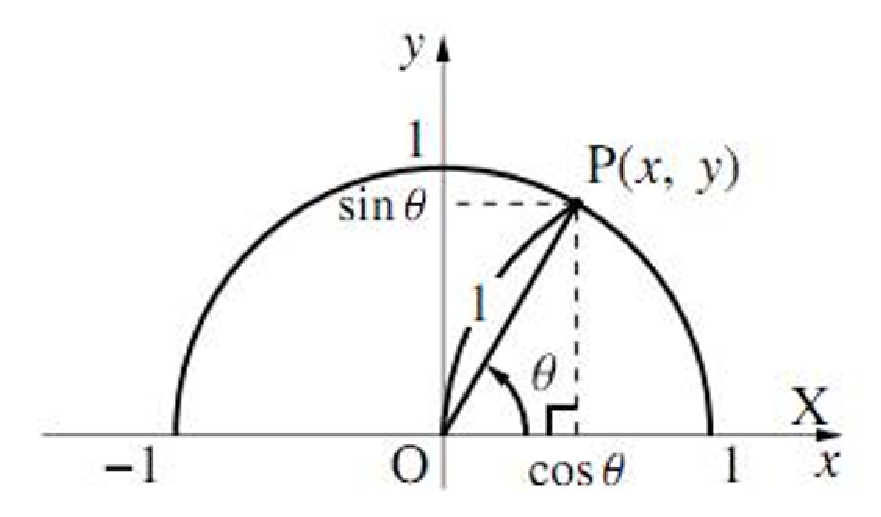
\includegraphics[width=10cm]{../figures/trigonometry.eps}
  \caption{三角比のイメージ図}
\end{figure}

\section{三角比の公式}
三角比には, いくつか公式があります. ここを暗記で片づけるのは阿呆のする事です. いったん確認してみましょう.
\begin{eqnarray}
\tan \theta = \frac{\sin\theta}{\cos\theta}
\label{eq:tan}
\end{eqnarray}
\begin{eqnarray}
\sin^2 \theta + \cos^2\theta = 1
\label{eq:square}
\end{eqnarray}
\begin{eqnarray}
\tan^2\theta + 1 = \frac{1}{\cos^2\theta}
\label{eq:tan2}
\end{eqnarray}
式(\ref{eq:tan})については自明ですね. 横の増加量分の縦の増加量なのだから, 傾きです.\\

式(\ref{eq:square})も自明です. ピタゴラスの定理です. 中2でやった. \\

式(\ref{eq:tan2})は一寸ややこしいですが, 式(\ref{eq:square})を用いれば秒で片づけられます. 式(\ref{eq:square})の両辺を $\cos^2\theta$ で割ったのが式(\ref{eq:tan2})です.\\

このように, 三角比の公式というのはおまじないではなく, 常識なのです. 感覚で理解し, すぐにその場で公式を作れるようにしましょう. 


\section{三角関数}
さて, 三角比がどんなものか分かったうえで, それぞれの三角比を関数として考えてみます.関数とは,ある変数の値によって定まる数の集合の事です.つまり$x$が1,2,3,...と値をかえていくにつれて変化していく$y$などを指し,$f(x)$などと表します.\\

 $\sin x $は$x$が$0 + 2\pi n$の時に0, $\frac{\pi}{2} + 2\pi n$の時に1, $\pi + 2\pi n$の時に0, $\frac{3}{2}\pi + 2\pi n$の時に-1を常に通り, その間を滑らかな曲線で結んだ関数になります. n の値は何周目かを表します.\\
\\
$\cos x $も同様にして1 ,0 ,-1 ,0 となっています. \\
\\
$\tan x$ は一寸特殊で, 三角形の斜辺の傾きを表すという性質上, 端がありません. よって x = 0の時には0, で正負方向に対称で$\frac{\pi}{2} + \pi n$で$\infty$ または $-\infty$ を極限としてとんでいきます.\\


ここまでは常識ですね?今時小学生でも知ってるかもしれません.\\

さて, こいつら三角関数の何がすごいかって, 超単純な周期関数である事です. \\

さらに, 実は sin と cos に限って言えば位相が違うだけでその形は全く同じなのです!!!みていてください.\\
\\
\begin{eqnarray}
\cos x = \sin (x + \pi/2)
\end{eqnarray}
こうなっているのでしたね.
\\

\begin{lstlisting}[caption=三角関数のMATLABコード,label=sc:tri]
t = (0:0.0005: 5)';
plot(sin(2*pi*1*t))
hold on
plot(cos(2*pi*1*t))
hold off
\end{lstlisting}


\begin{figure}[H]
\label{im:sincos}
  \centering
  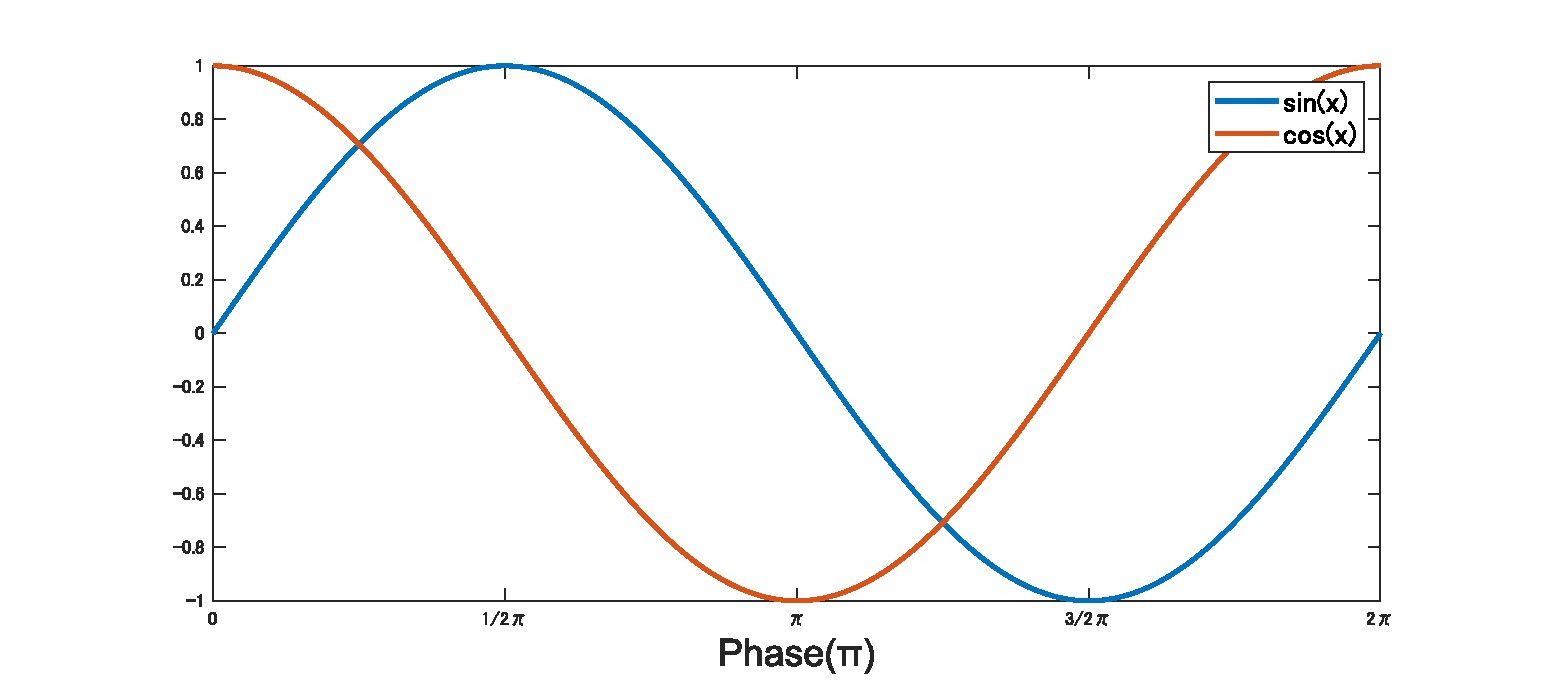
\includegraphics[width=15cm]{../figures/sincos.eps}
  \caption{sin / cosの図}
\end{figure}

\section{加法定理\label{addition_theorem}}
これはオイラーの公式を用いる事で, 覚えていなくてもその場で導出できます. (オイラーの証明(参照: analysis)) みててください. オイラーの公式より
\begin{eqnarray}
\mathrm{e}^{i(\alpha + \beta)} = \cos (\alpha + \beta) + i\sin (\alpha + \beta)
\label{eq:aplusb}
\end{eqnarray}
指数法則より,
\begin{align}
\mathrm{e}^{i(\alpha + \beta)} &= \mathrm{e}^{i\alpha} + \mathrm{e}^{i\beta} \\ &= (\cos \alpha + i\sin\alpha)(\cos\beta + i\sin\beta) \\
&= (\cos\alpha\cos\beta - \sin\alpha\sin\beta)\pm i(\sin\alpha\cos\beta + \cos\alpha\sin\beta)
\label{eq:kahou}
\end{align}

ここで再び式(\ref{eq:aplusb})と見比べると, 式(\ref{eq:kahou})の実部がcos, 虚部がsinの加法になっている事が分かります. ここから三角関数の加法定理は


\begin{eqnarray}
\sin (\alpha + \beta) = (\sin\alpha\cos\beta + \cos\alpha\sin\beta)\\
\cos (\alpha + \beta) = (\cos\alpha\cos\beta - \sin\alpha\sin\beta)
\label{kahouteiri}
\end{eqnarray}

と証明できます. 例のごとくtanは一寸面倒なので, 自分で証明してみてください.
\section{正弦と余弦}
sinとcosの関数の定義は分かりましたが, それがなんで嬉しいのでしょうか?\\
これを知るためには, sinとcosの関係はどんなものであるのか考える必要があります.\\
\\
ここで前回やった掛け算が出てきます. \\
任意のsin関数とcos関数の積を考えてみます.\\
\\
$r_1\sin mx $と $r_2\cos nx $です.\\
\\
ここで$r_1$, $r_2$は振幅, mとnは角周波数を示していますので, 異なる周波数の三角関数になっています.\\

\begin{figure}[H]
\label{im:sines}
  \centering
  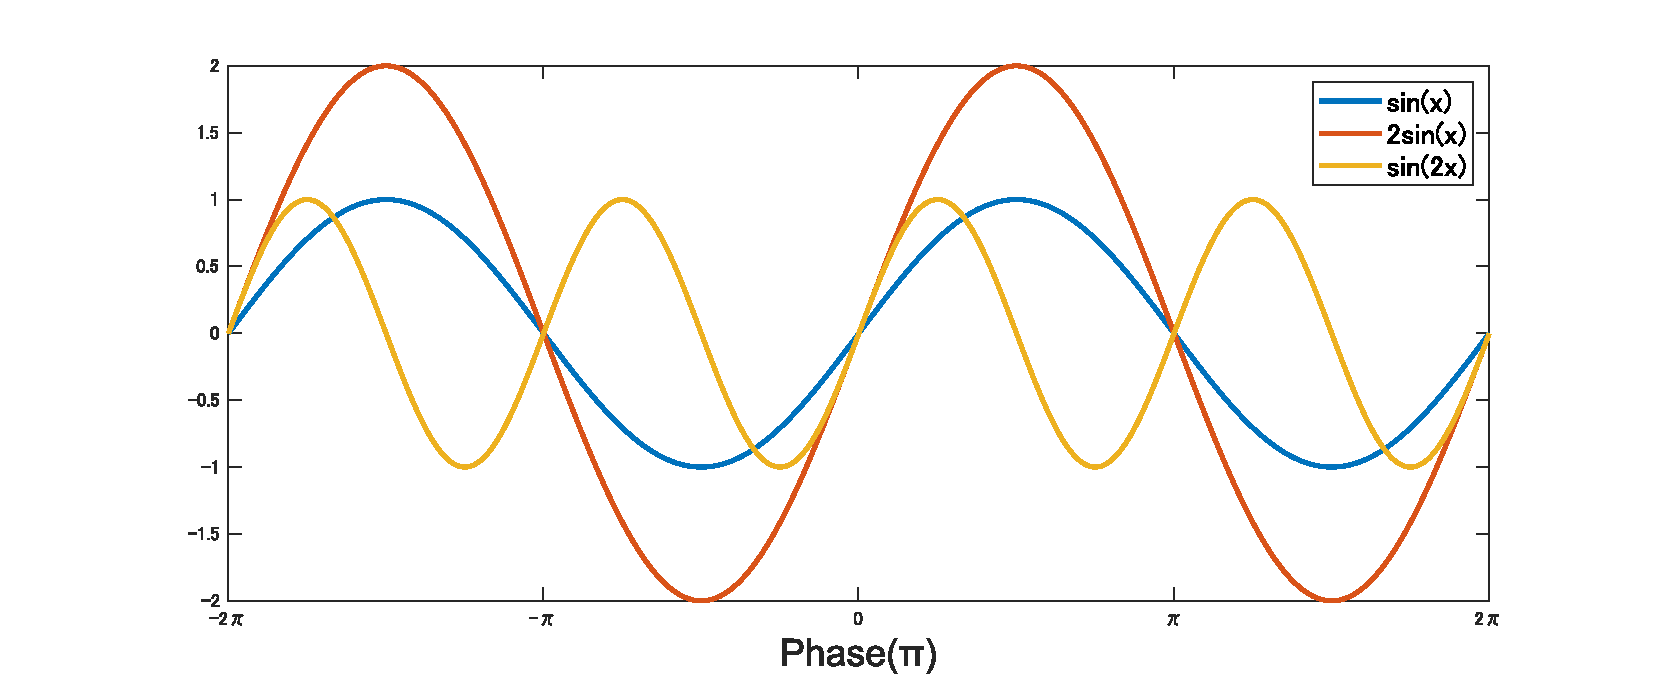
\includegraphics[width=15cm]{../figures/sines.eps}
  \caption{様々なsin波の図}
\end{figure}

こいつらの掛け算を考え, さらにそいつを積分してみます.\\
\\
\begin{eqnarray}
\label{eq:cosint}
  \int^\infty_{-\infty} r_1\sin mx r_2\cos nx dx = \int^{2\pi}_0 r_1\sin mx r_2\cos nx dx = 0
\end{eqnarray}
\\
三角関数は $2\pi$周期で同じ波形の繰り返しになっているので, 範囲が$\infty$ から$-\infty$じゃなくていいのは自明ですね.\\
\\
三角関数は周期関数なので, それぞれが積分すると0なのも自明ですが, 更に積の積分も0になるのです!!!\\
これはすごい!!波としては複雑になっても, 周期関数である事に変わりはなく, 積分しても0になるのは変わらないわけです!!\\

\begin{lstlisting}[caption=式(\ref{eq:cosint})あたりのコード,label=sc:cosint, keepspaces=true, language=Matlab]
syms x         // シンボリック変数
int(cos(x), [0 2*pi])       // 0 -- 2pi の積分,どちらも当然 0
int(sin(x), [0 2*pi])
int((2*(sin(3*x))*(3*cos(10*x))), [0 2*pi])  // [r1 r2 m n] = [2 3 3 10] の 0--2pi の積分. これも 0
\end{lstlisting}

\section{関数の内積 \label{dot}}
さて, ここで掛け算の復習です. ベクトルの演算, ドット積の定義を覚えていますか?\\
\\
そう, 対応する次元の要素を掛け合わせたものの総和でしたね!\\
\\
これ...関数でも使えそうじゃないですか!?\\
同じxの値の時のy同士をかけ, それの足し合わせをするのもやってる事は同じなのです!!\\
\\
\\
これを使うと, すごい事がおきます. そう. 関数に内積を定義できるのです!!すばらしい!!\\
ただし注意する必要があるのは, ベクトルでは総和をΣで表していましたが, 関数の場合はxが離散値ではなく連続値(参照: \ref{ed})をとるため, 総和はΣでなく∫で表す(参照: \ref{convolution})という事です.\\
\\
いずれにせよ, 掛け算の総和で関数の内積を定義できる事に変わりはないです. これは崇める必要がありそうですね!!\\
この節の話題から少し離れてしまうため, 細かい解説は\ref{dot_func}へ飛ばします. 大事なのは, 関数でも内積が定義できるという事です.


\section{関数の直行性}
話をもどします. ベクトルにおいて内積が0になるとどうなっていましたか?\\
そう, 直交です!!!\\
\\
ベクトルの内積を関数の内積に拡張する事ができ, ベクトルの内積が0という事は直交を表す...すなわち関数についても直行性を定義する事が出来るのです.\\
\\
sinとcosは直交する関数なんですね!!!すごい!!\\
ここでよくある勘違いについて言及しておくと, 直交と直角は別物です. 留意せよ.
\section{直交性}
ここでは関数の直行性については細かい話は省きますが, 直交する関数2つ(sinとcos)を用意できたなら, これを使えばすべての関数を表す事が出来ます.\\
\\
そりゃそうですよねー. 複素数や直交座標系と同じノリです.\\
\\
つまり...全ての(周期)関数は, 異なる振幅, 周波数の三角関数の足し合わせによって表す事ができるのです!!!\\

\begin{figure}[H]
\label{im:furier}
  \centering
  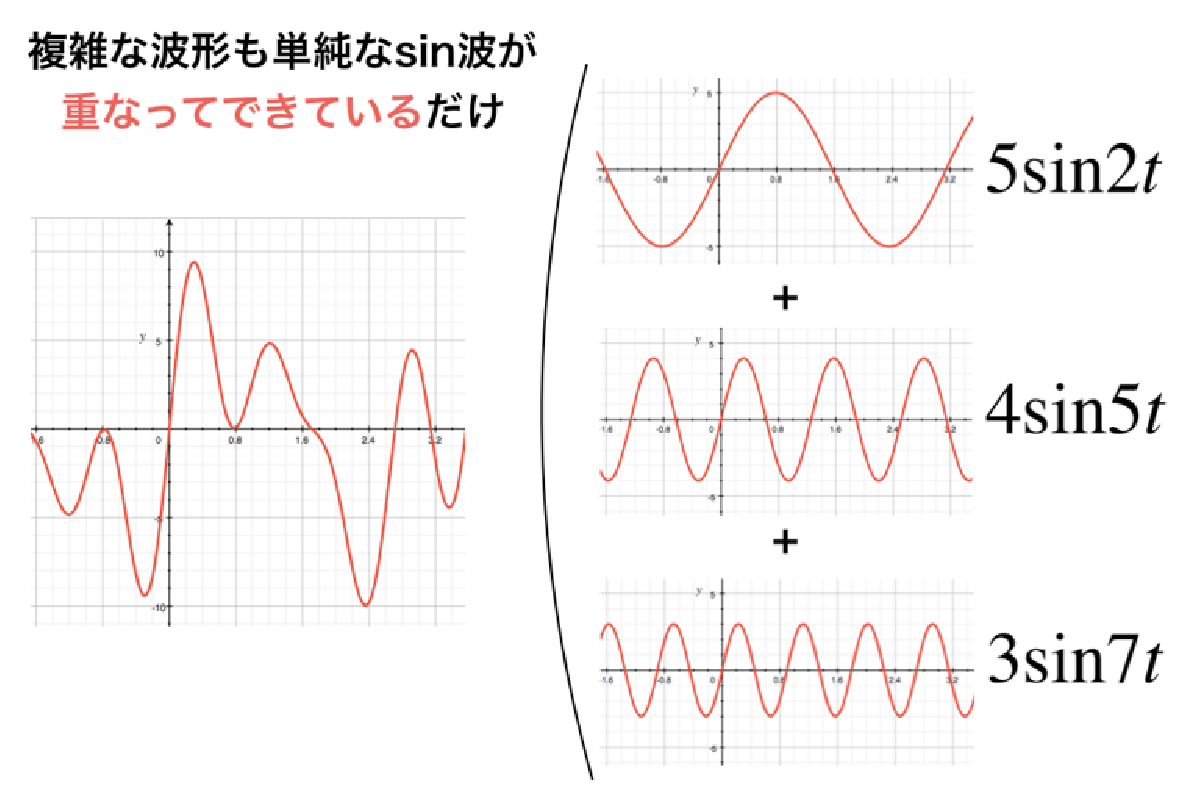
\includegraphics[width=10cm]{../figures/furier.eps}
  \caption{フーリエ変換の気持ち (宇宙一分かりやすいフーリエ変換より)}
\end{figure}

\subsection{フーリエ変換への一歩}
前項での内容を式に表すとこうなります. よく見てください.
\begin{eqnarray}
f(x) = \sum_{n=1}^\infty ({a_n \sin(\omega t) + b_n\cos(\omega t)}
\label{eq:sum1})
\end{eqnarray}
ここで, 式(\ref{eq:sum1})はすべてsin,cosの値が0になる角度の際に吐き出される値も0になるものですが, 実世界においてはそううまくはいかず, そもそもこの関数の背景にある信号の影響によって基準値が上昇します. 電気回路系で言うなら直流電源などです.そこで式(\ref{eq:sum1})を改造します.

\begin{eqnarray}
f(x) = a_0 + \sum_{n=1}^\infty ({a_n \sin(nt) + b_n\cos(nt)}
\label{eq:fixed_sum})
\end{eqnarray}

ここで$a_0$はDC電源の分です.\\
\\
脳波は時間によって変化する時間関数ととらえる事が出来るので, この方法で脳波を三角関数に分解して表現する事が出来るのです!!!\\
\\
これが三角関数を崇める理由です.\\
\\
そしてこの, 時間関数f(t)を三角関数の和に変換する事をフーリエ変換といいます. 詳しくは今度(Advanced).\\
\section{大正義オイラーの利用}
とはいえ, 三角関数を$\infty$に足し合わせるというのも酷な話で, 計算が面倒なこと面倒なこと...\\
\\
どうにかならんもんか...\\
\\
ん?三角関数の足し合わせ? どこかで聞きましたね?\\
そう, 式(\ref{eq:euler})に表した, 我らが至宝オイラーの公式です!!!\\
\\
オイラーの公式を用いる事で, 三角関数の足し合わせは指数関数で表せます. これを使う事で劇的に計算を楽にする事ができるのです!\\
ただ, オイラーの公式にはsinの前に謎の記号 i がついています. 一体こいつはなんなのでしょう. 次の章では, 虚数と複素数について学びます.\\

\chapter{複素数}
複素数とは偉大なものでありますが, 最初は理解に非常に苦しむものです. ですが複素数をマスターするという事は, 整数から分数への拡張や, 正の数から負の数への拡張を遥かにしのぐ恩恵を与えてくれるのです. 高校で習う内容ですが, ここでもう一寸深く学んでみましょう!\\
\section{虚数}
虚数の定義からおさらいをしましょう. 高校で習う領域の中でも, 比較的簡単だったはずです.\\
\\
虚数とは, 平方すると-1になる数を基底とした数の事です.\\
\\
1本の直線でしかない実数の問題は, 表現の幅が圧倒的に限られてしまう事です. そこで昔の人類は, 実数軸を2本直角に重ね合わせた直交座標系やベクトルといった考えを用いたわけです.\\
\\
しかし, 虚数の登場がこの常識を大きく変える事になりました!!\\
\\
ベクトルあるいは行列を少し復習しましょう.\\
これらにおいて, 次元はどうやって定義されていたでしょうか? 直交性・独立性ですね!!!\\
\\
実数ではない...正確には,0の時(つまり交点)以外に必ず実数と交わらず, 直交性をもった「数」を定義できないか?
昔の偉い人はこう考えたのです. 頭おかしいですね!!\\
\\
こうして生まれたのが虚数単位iです. 実数において単位として利用される1の概念と直交する必要があったため, ここで1の平方が1である事に注目しました. \\
\\
平方して負の値になる数は存在しない. これは中学で習う事ですがこれを厳密に言うと, 「従来の数には存在しない」と解釈したわけです.\\
\\
そこで, 平方して負の値になる数を考え, これを虚数と名付けました.\\
実数の単位が1なら, 虚数の単位は1iとなります. 虚数も0の平方にマイナスをつけようとしたところで0なので, 実数と虚数は0で直交する事になります.\\
\\
これが虚数の定義ですね!! 高校数学では「存在しない数」などと習いますがこれは誤解を招きます. 虚数の意義とは「y軸」を定義できる事にこそあるのです!!!\\
存在しない数があったから, 虚数と名付けたのではなく, 実数と直交性を持った数 = 虚数として使えそうな定義はないものかと考えた時に, 平方すると -1 になる数, を考え付いたわけです.

\section{虚数の性質}
虚数は単位iがついてるだけなので, 基本的な足し算引き算はすべて実数と同様に扱えます. 簡単ですね!\\
\begin{eqnarray}
\label{eq:implus}
3i + 5i  =(3 + 5)i = 8i
\end{eqnarray}
掛け算になると一寸難しくなり, 虚数同士をかけると数字同士の積にマイナスをつける必要があります. それが虚数の性質でしたね!\\
\begin{eqnarray}
\label{eq:imkake}
3i \times 5i = (3\times 5)i^2 = 15 \times -1 = -15
\end{eqnarray}


\begin{lstlisting}[caption=式(\ref{eq:implus} \ref{eq:imkake})あたりのコード,label=sc:imcal , keepspaces=true]
3*1i + 5*1i        // add
3*1i * 5*1i        // multiply
\end{lstlisting}

コード(\ref{sc:imcal})ではそもそも虚数単位と数字を分けて書いてますね,こう書かれると数字と虚数単位を別に計算させてるのもより実感できます.余談ですが,プログラムを書くときは変数のiとかと混ざらないようにこのような記法をして虚数単位を区別する書き方が推奨されています.この掛け算, 実は複素数の掛け算の性質を考えると自明になります.\\
この章の最後でそれを説明します!\\
\section{複素数}
虚数のおさらいができたところで, 複素数です. 実数も虚数も直線であるため, これらを軸として, 直交座標系っぽいものを考えます.\\
\\
こうしてできた平面の事を, 複素平面やガウス平面といいます.\\
\\
さて, ガウス平面を考えた際, とてもうれしい事が数多くあります. まずはそれぞれの軸における長さですが, 実数も虚数も単位が1(i)であるため, 原点からの距離を考えると $ |a| = |ai| $ になっているのです. \\
\\
この性質を利用すると, ガウス平面上の任意の点をユークリッド平面(今まで見た事のある関数のグラフのあれ)の点に対応づける事ができ, (x, y) ≒ x + yi といった具合に表す事が出来ます. \\
\\
何故ユークリッド平面では(x,y)なのにガウス平面だと足し算で表せるのか?ユークリッドはxもyも実数だけど,ガウスの場合は実数と虚数で独立しているからです.これがやりたいから虚数を考えたのでしたね!\\
\\
このように, 実数部分と虚数部分の足し合わせによって, 複素平面(二次元)上の数を表現した数を複素数といいます.\\
\\
こいつのうれしさは, 直交座標や行列のように複数の数の集まりではなく, ひとつの数として扱える点です!!!\\

\begin{figure}[H]
\label{im:imagine}
  \centering
  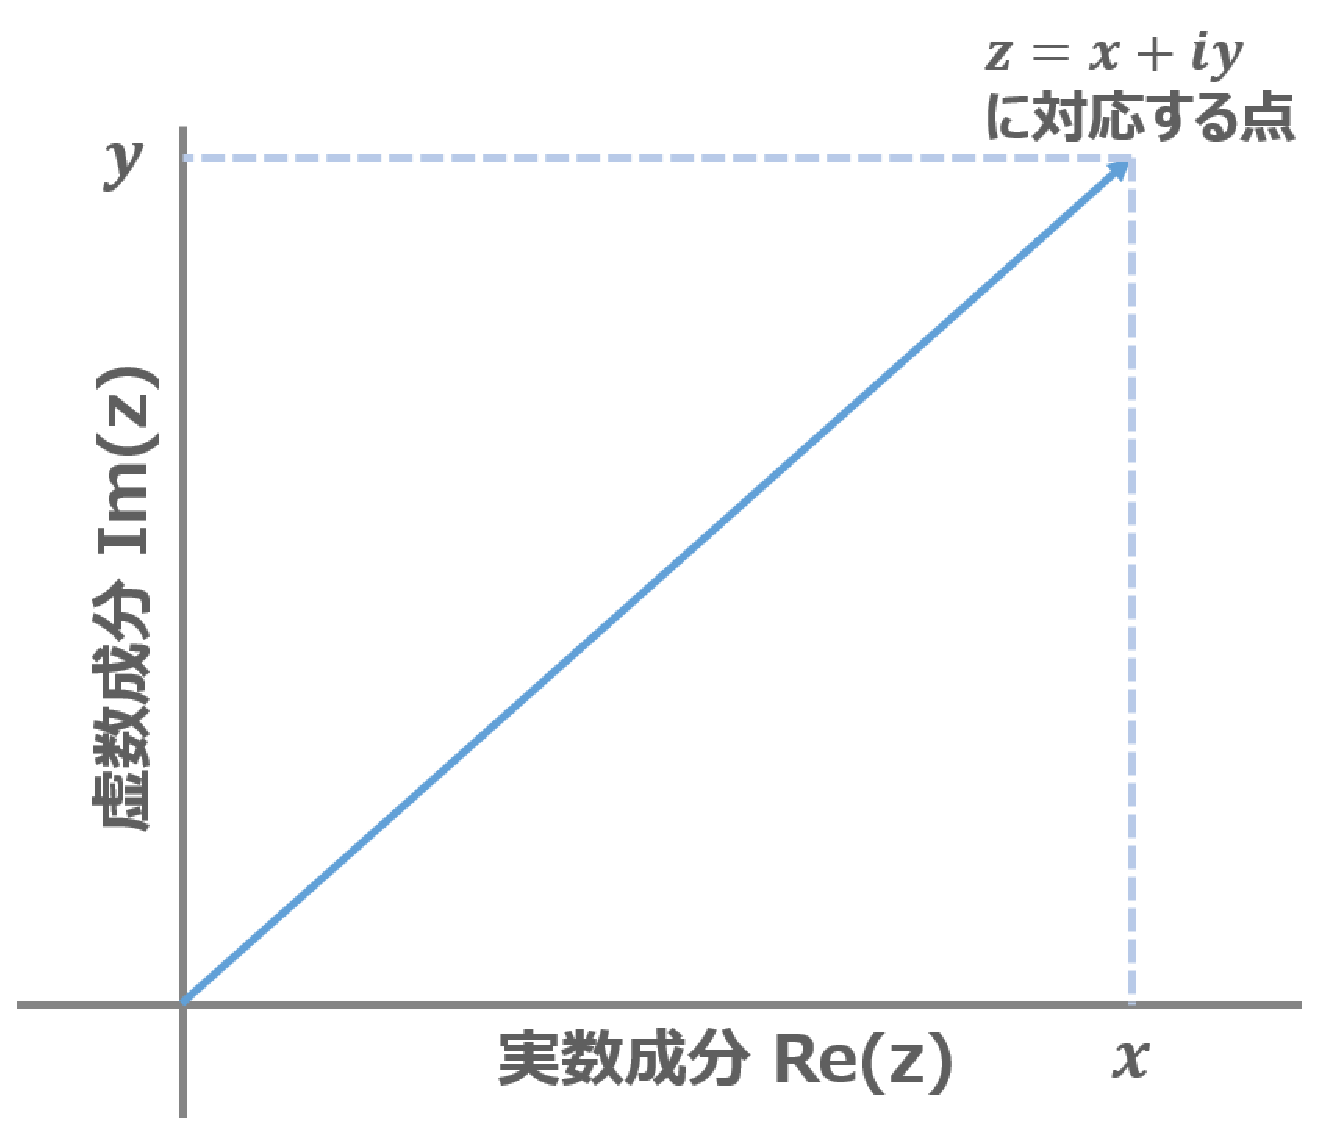
\includegraphics[width=10cm]{../figures/gauss.eps}
  \caption{複素数}
\end{figure}

\section{数の大幅な拡張}
複素数の定義が分かったところで, これが実際にどうやって影響してくるのかについて考えます. 一次元が二次元に拡張されたわけですからその恩恵は計り知れません. \\
\\
さらに複素数の偉大な点は, 実数を複素数の一部として扱える点です.\\
\\
たとえば3は, 複素数で表すと 3 + 0iとなります.\\
そして注意しないといけないのは, 複素数を実数に変換した場合, その虚数成分は捨てられてしまうのです!!\\
実軸に投射される過程で, 虚軸(高さ)成分は消えてしまうという事です.\\
\\
つまり...\\
我々が今まで3だと思ってた数は, 実は 3 + 5i かもしれない...という考え方もできます!!\\
\\
ちょっと違うような気もしますが, たとえば大学の単位で考えましょう.\\
成績がCでもSでも, 来る単位は1です.\\
\\
実軸を単位, 虚軸を成績とすると, 実軸だけではCの人もSの人も同じ優秀さぽく見えますが, 虚数成分も合わせれば同じ単位取得者でも上下関係があった事に気付けるわけです!!\\
\\
まぁ,今のたとえ,成績と単位は線形独立でないので本当はだめですが,まぁイメージとしてはそんな感じという事で目を瞑ってください.
\\
とかく,複素数は偉大ですね!!
\\
実はこの考え方が後にウェーブレット変換を学ぶ際に非常に重要になるのです. 頭の片隅においておいてください.\\

\section{複素数平面}
複素数平面において, 任意の点 x + yi を表す方法について考えていきます. \\
\\
実軸と虚軸の直行性より, 複素数 z = x + yi の横(実部Re)の長さ(\ref{eq:x})と, 縦(虚部Im)の長さ(\ref{eq:y}), 原点との距離(\ref{eq:length}), そして実軸との間になす角(\ref{eq:arg})はそれぞれ
\begin{eqnarray}
\label{eq:vector}
\mathstrut Re z = x
\label{eq:x}
\\
\mathstrut Im z = y
\label{eq:y}
\\
|z| = \sqrt{x^2 + y^2}
\label{eq:length}\\
\mathstrut arg z = \tan^{-1} \frac{y}{x}
\label{eq:arg}
\end{eqnarray}
のように表されます. 長さについては直交座標なので自明ですね. 絶対値に関してもピタゴラスの定理より自明. 式(\ref{eq:arg})で表される角の事は, 偏角と言います. 実軸との角度の事であるので, tanを使って表す事が出来るというわけですね.\\

また, 複素数 z を実軸に線対称な点を取った点の事を $ \overline{z}$ と表し, 複素共役な点といいます.\\

\begin{eqnarray}
\label{eq:conj}
z = x + yi
\end{eqnarray}
\begin{eqnarray}
\overline{z} = x - yi
\end{eqnarray}

\begin{figure}[H]
\label{im:complex}
  \centering
  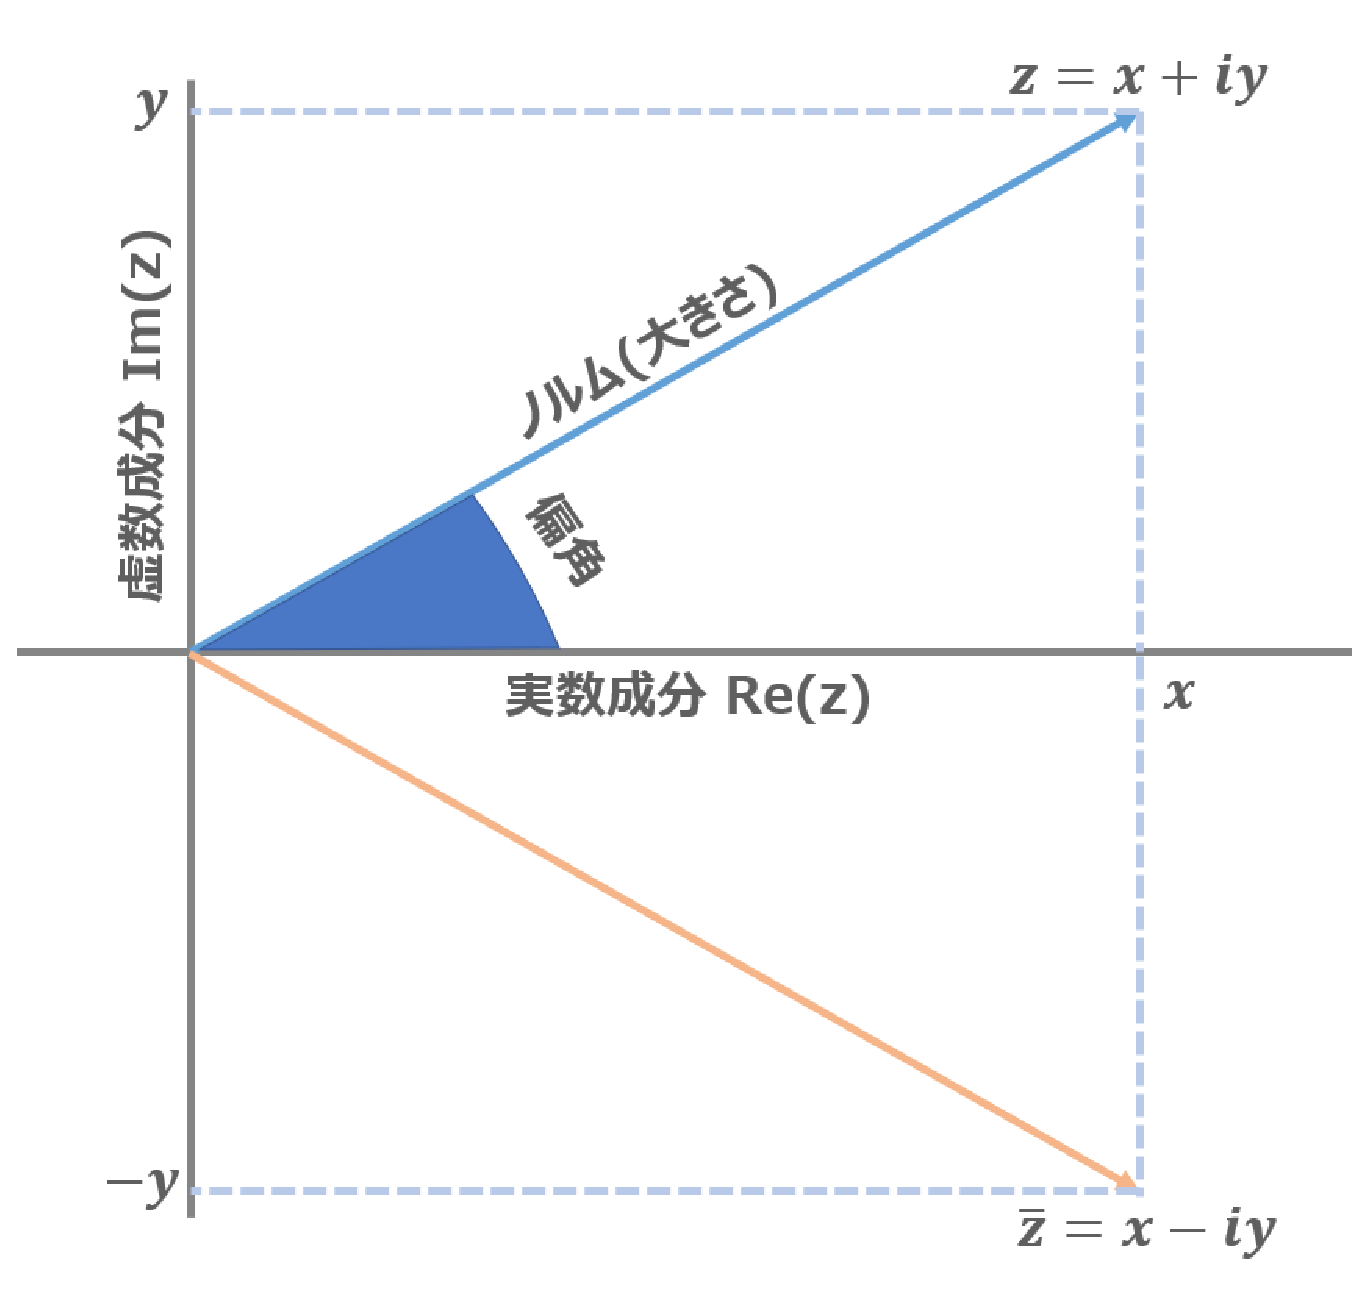
\includegraphics[width=10cm]{../figures/Complex.eps}
  \caption{複素平面}
\end{figure}
MATLABではそれぞれ,以下のようにして求める事が出来ます.

\begin{lstlisting}[caption=式(\ref{eq:vector}\ref{eq:conj})あたりのコード,label=sc:vector]
x = 3 + 4*1i
real(x)        // 実部
imag(x)        // 虚部
abs(x)        // ノルム,絶対値
angle(x)        // 偏角
conj(x)        // 複素共役
\end{lstlisting}

\section{極形式}
複素数 z は x + yi のような表記の仕方以外に, もう一つの表し方ができます.\\
\\
前節で確認した, 複素数 z の絶対値は, 原点との距離を表す実数でした. 範囲は0以上の実数になりますね!!\\
\\
偏角の取りうる範囲はどうなるでしょうか?\\
原点を中心として4つの象限をぐるぐる回るので, -π ~ πですね!\\
\\
\\
この2つに注目して考えます. 原点からの距離(r)と偏角($\varphi$)が分かるという事は, 平面上で一意に定まる点を定義できますよね?三角比でcosは横,sinは縦の長さでした.
\begin{eqnarray}
z = x + iy = r(\cos \varphi + i\sin \varphi)
\label{eq:kyoku}
\end{eqnarray}

$r\sin\varphi$ で導出される数は実数(y)になっているため i をかける事を忘れないように.\\

\begin{figure}[H]
\label{im:polar}
  \centering
  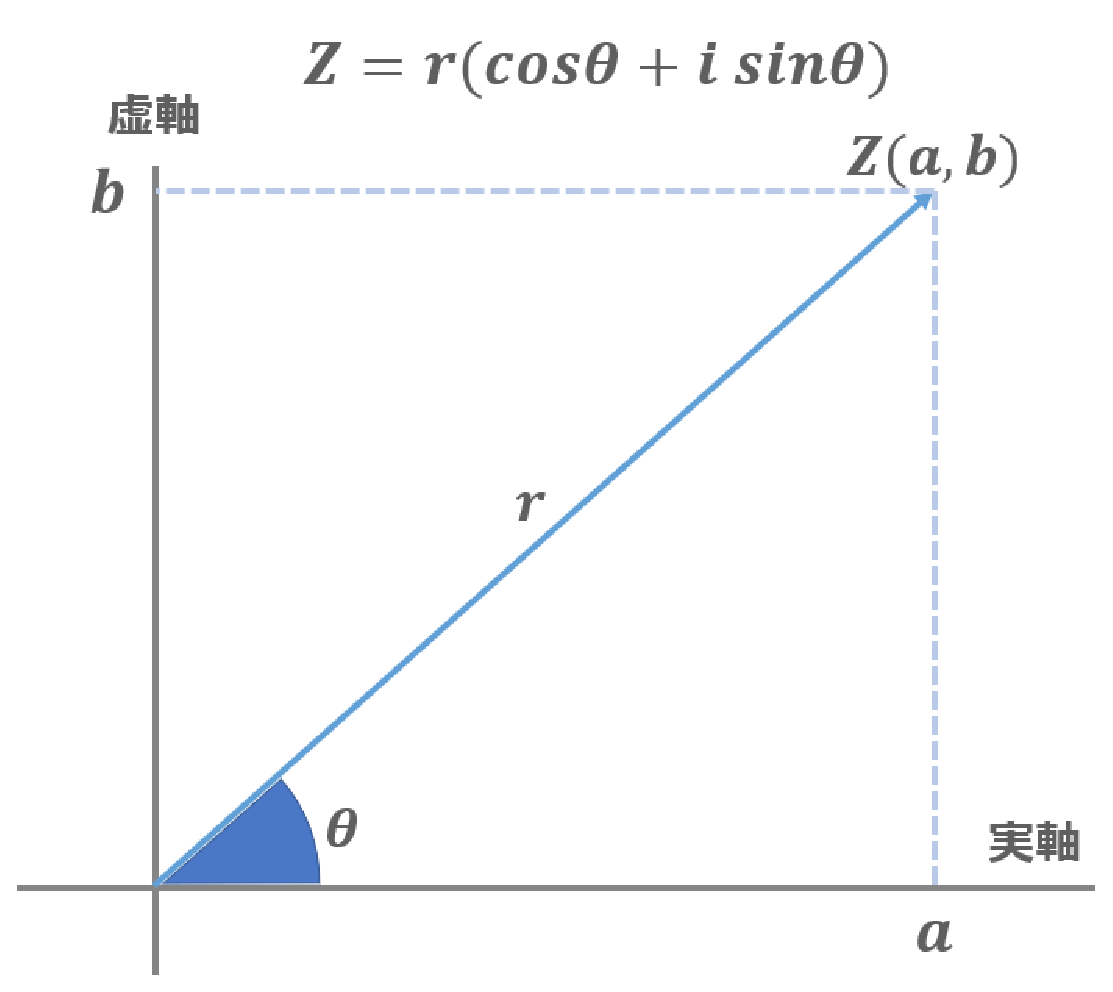
\includegraphics[width=10cm]{../figures/polar.eps}
  \caption{極形式の視覚的理解}
\end{figure}

\section{大正義オイラー再び}
式(\ref{eq:kyoku})の最右辺をよく見てください. どこかで見た式ですね!!!\\
人類の至宝を利用する事により式(\ref{eq:kyoku})はこのように変換する事が出来ます.\\
\begin{eqnarray}
z = x + iy = r(\cos\varphi + i\sin \varphi) = r \mathrm{e}^{i\varphi}
\end{eqnarray}

\section{複素数の掛け算}
さて, 複素数を $r\mathrm{e}^{i\varphi}$ で表せたところで, 複素数の掛け算を改めて考えます.\\
\begin{align}
z_1 z_2\\
& = (x_1 + iy_1)(x_2 + iy_2) = (x_1 x_2 - y_1 y_2) + i(x_1 y_2 +x_2 y_1)\\
&= r_1(\cos\theta_1 + i\sin\theta_1)r_2(\cos\theta_2 + i\sin\theta_2)\\
&= r_1r_2\mathrm{e}^{i\theta_1} \mathrm{e}^{i\theta_2}\\
&= r_1r_2\mathrm{e}^{i(\theta_1 + \theta_2)}
\end{align}

こうなっているのです!!!\\
複素数の掛け算は絶対値をかけた上の回転を表すのですね!!
\section{戻り学習}
ここで再び, 虚数とは何か, 何故平方すると-1になるのかを考えます.\\
任意の複素数を考えます. ここでは面倒なので $ 3 + 0i$ としましょうか.
\begin{eqnarray}
3 + 0i = 3(\cos 0 + i\sin 0) = 3(1 + 0) = 3
\end{eqnarray}
こんな感じに表せますね.\\
こいつに0+1iをかけます. よく見ててください.
\begin{eqnarray}
i(3 + 0i) = 3i(\cos 0 + i\sin 0) = 3i(1+0) = 3i\\
\end{eqnarray}
そしてこいつと...
\begin{eqnarray}
3(\cos (0+\frac{\pi}{2}) + i\sin (0 + \frac{\pi}{2})) = 3(\cos\frac{\pi}{2} + i\sin\frac{\pi}{2}) = 3i
\label{eq:roll}
\end{eqnarray}
こいつを見比べるのです. 同じ値になってますね!!\\
複素数の積は回転を表すので, つまり i をかけるという事は $\frac{\pi}{2}$ 回転するという事なのです!!\\
\\
なのでもちろん式(\ref{eq:roll})にiをかけると, -3 になります. 虚数単位i を2回かけると-1を掛ける事になる, つまり $\pi$ 回転するのですね!\\
まだしっくりこないなら,たとえば$cos0\pi = 1$は$\frac{\pi}{2}$回転すると0になり, もう一度かけると -1になりましたね?実数である1が消え(虚数では存在してる),再び実数にもどってきたというわけです.
\section{まとめ}
このように三角関数と虚数は非常に親和性が高く, そしてオイラーの公式によって指数関数ともつながる非常に重要な概念になっています. \\
\\
三角関数と虚数を理解すれば, 脳波解析を学ぶ基礎となる数学はほぼ出そろったという事になります!!\\
しっかりと理解していってください!!\\

\chapter{微分・積分}
この章ではみんな大好き微分積分いい気分の気持ちを考えていきます.\\
高校数学で習うなかでも, とびっきり意味が分からない分野ですね.\\
\section{極限とは}
まず, 微分や積分といった計算は超極小の範囲で考える数学です. この超極小というのがなんなのかから考えます.\\
\\
超極小...曖昧な響きですね. 我々の身長の話をしている際にmmを持ってきたら極小と言えますが, 蟻の体長の話をしている時には大きすぎますね. \\
\\
このように, どんなスケールでの話をしていても十分に小さいといえるようなスケールでの話が微分積分です.\\
\\
実用では「0に限りなく近づく」などといった表現で表され, 数式だとこうなります.
\begin{eqnarray}
\lim_{x\to0} f(x)
\end{eqnarray}
この意味するところは, 関数f(x)のxを限りなく0に近付けた時の関数の返す値という事になります. つまり f(x) が 2x とかであれば
\begin{eqnarray}
\lim_{x\to0} 2x \fallingdotseq 0
\end{eqnarray}
になります. しかしここでxは限りなく0に近い値なので実質的にはこの式が返す値も0と見做せるので, 等号は成り立ち, 点々は外れます.
\begin{eqnarray}
\lim_{x\to0} 2x = 0\\
\lim_{z\to\infty} 2x = \infty
\end{eqnarray}
\section{ε-δ論法 \label{ed}}
限りなく0に近いって曖昧な表現ですよね. さっきも言ったようにmmなのかμmなのか, どこからが限りないと言っていいのかわかりません. ここで極限


\begin{eqnarray}
\lim_{x\to a} f(x) = b
\end{eqnarray}
は数学語では


\begin{screen}
ε-δ論法
\begin{eqnarray}
\forall \varepsilon >0, \exists \delta>0  s.t.  \forall x \in \mathbb{R}, |x-a|<\delta \Rightarrow |f(x)-f(a)|<\varepsilon
\label{eq:ed}
\end{eqnarray}
\end{screen}

のように定義されます. 有名な$\varepsilon - \delta $論法というやつです.\\
\\
この式の意味はこうです.\\
\\
任意の正の数$\varepsilon $に対し, ある適当な正の数$\delta$が存在し, $0<|x-a|<\delta$ を満たす全ての実数xに対し,$|f(x)-b|<\varepsilon$ が成り立つ.\\
\\
f(x)とbの間の距離が任意の正の数εより狭い範囲において, 必ず対応するxの値が存在しているといった具合で, 「お前がどんなに頑張ろうと俺はその上をいく」みたいなやつです. これが連続値の定義になるわけですね.

\begin{figure}[H]
\label{im:ed}
  \centering
  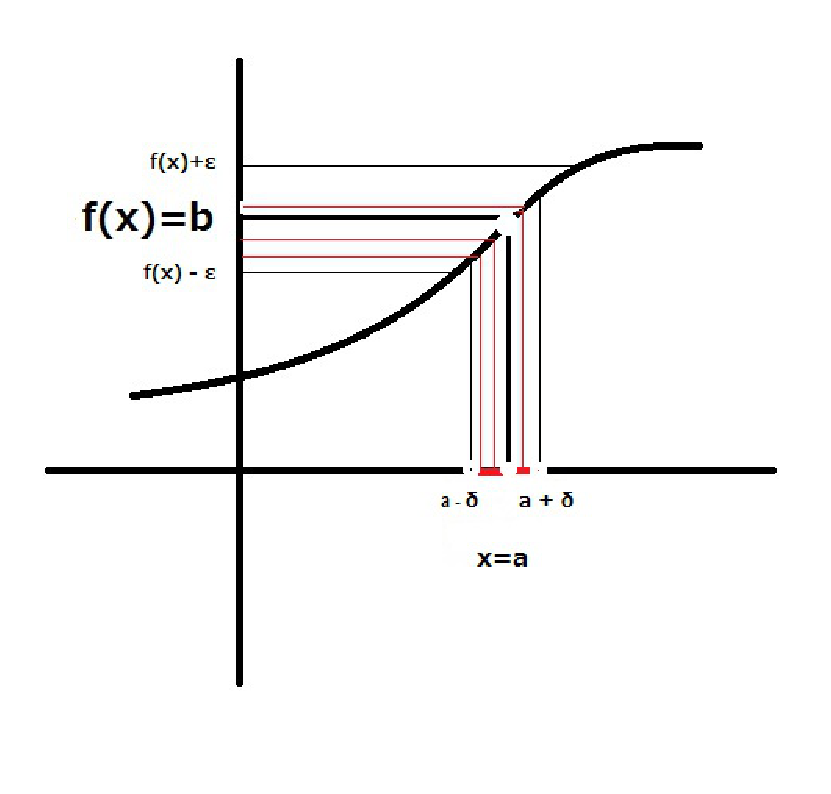
\includegraphics[width=10cm]{../figures/ed.eps}
  \caption{ε-δ論法. aの左側は連続だが右は連続じゃない}
\end{figure}

つまり極限とはmmなのかμmなのか?という問いに対する答えは, 「お前がmの話をするならcm, cmの話をするならmm, mmの話をするなら...」を死ぬまでやるイタチごっこだということです!!\\
\\
ちなみに式(\ref{eq:ed})はついでに関数の連続性についても定義していて, どんなに小さい範囲で見てもそれより小さい値が存在するという事は切れ目なくしっかりとつながっている=連続であるという定義にもなります.\\
\section{微分}
\subsection{微小な変化率}
さて, 極限とはある一点に限りなく小さい範囲を考える事でした.\\
ここで, 関数でも同じ事を考えます.\\

関数とは,ある変数の値によって定まる数,その式(e.g. $y = f(x)$)の事でした.微分とは言ってしまえば変数の変化を極限まで小さくした時,関数の値はどの程度動くか,という割合を求める操作の事です.先に式を見せます.

\begin{eqnarray}
\label{eq:prime}
f'(x) =\lim_{dx \rightarrow 0} \frac{f(x+dx) - f(x)}{dx}
\end{eqnarray}

$x$をdxだけ動かしたときの$y$の変化率ですね.思い出してほしいのは中学数学で二点間の傾きを求める式です.関数の時にやりましたよね.

\begin{eqnarray}
\text{傾き} = \frac{y\text{の変化量}}{x\text{の変化量}} = \frac{f(x_2) - f(x_1)}{x_2 - x_1}
\end{eqnarray}

ってやつです.これを,$x$の変化量を限りなく小さくした版が式(\ref{eq:prime})です.良いでしょうか.つまりその一点での傾き,接戦を求める式になっているわけですね.高校の時に微分とは接戦を求める操作であるなんて習いました.ちょっとその説明は良くない気がして,あくまで接戦を求める操作にもなるってだけで本質は「関数の局所的な微小変化率を求める事」です.\\

\begin{figure}[H]
\label{im:sessen}
  \centering
  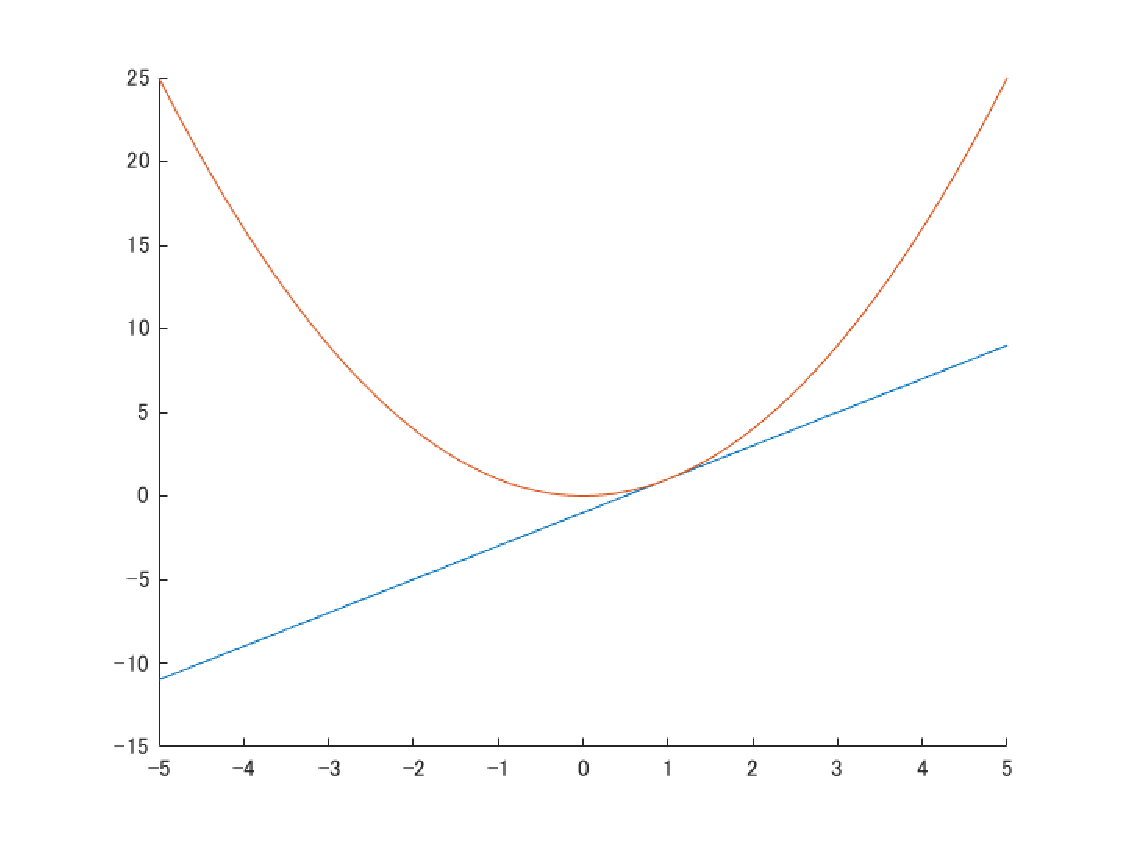
\includegraphics[width=10cm]{../figures/sessen.eps}
  \caption{局所的な微小変化率 = 接線?}
\end{figure}

また,関数$y=f(x)$の微分は本やサイトによって様々な記法があります.以下はすべて同じです.

\begin{eqnarray}
f'(x) = y' = \frac{dy}{dx} = \frac{df}{dx} = \frac{d}{dx}f = \frac{d}{dx}f(x)\nonumber
\end{eqnarray}

面倒ですね...分野によったりしても好まれるのが違うので,適宜使い分けていく事になります.このシリーズでもいくつかの記法を使っていると思います.
\subsection{三角関数の微分}
上記の性質が分かっていれば, 簡単な公式達です. 覚えるまでもありません.
\begin{eqnarray}
(\sin x)' = \cos x \\
(\cos x)' = -\sin x \\
(-\sin x)' = -\cos x \\
(-\cos x)' = \sin x
\end{eqnarray}

\begin{lstlisting}[caption=いろんな微分,label=sc:diff]
syms x
diff(cos(x))
diff(cos(x)*(sin(x)))
diff(exp(x))
\end{lstlisting}
自明ですね. sin, cos関数それぞれがどういった挙動をしていて, その傾きをすべての点で取ってつなげていったらどうなるかを考えれば, 自ずと分かるはずです.\\
\\
「微分とは, 局所的な微小変化率を求める事」です.\\
\subsection{ネイピア数}
三角関数の次, 微分といったらこいつですよね. πと並び超越数として名高い e の出番です.\\
ネイピア数は別名オイラー数です. これだけで崇めないといけない気がしてきますね!?\\
\\
$(\mathrm{e}^x)' = \mathrm{e}^x$ つまり, 指数関数にしたときに微分しても値が変わらないという変態な数です.\\
\\
微分しても値が変わらないって, わけがわからないですよね. 微分とは傾きを求める事だとか, 体積から面積を求める事, といった理解をしていると全く訳がわからなくなります.\\
\begin{eqnarray}
e = \lim_{x\to 0} (1+x)^\frac{1}{x} = \lim_{x \to \infty} (1+\frac{1}{x})^x
\end{eqnarray}
定義としてはこんな感じです.\\
まぁここは良いです. 大事なのは指数関数を微分しても値が変わらないという性質の確認だけです.\\
\\
さて, 一般に正の1以上の数を底とする指数関数は, 第一象限で二次関数的な上がり方をし, (0,1)を通って, 第二象限ではx軸に漸近しつつ徐々に横ばいな形をとりますね?\\
\begin{figure}[H]
\label{im:sisuu}
  \centering
  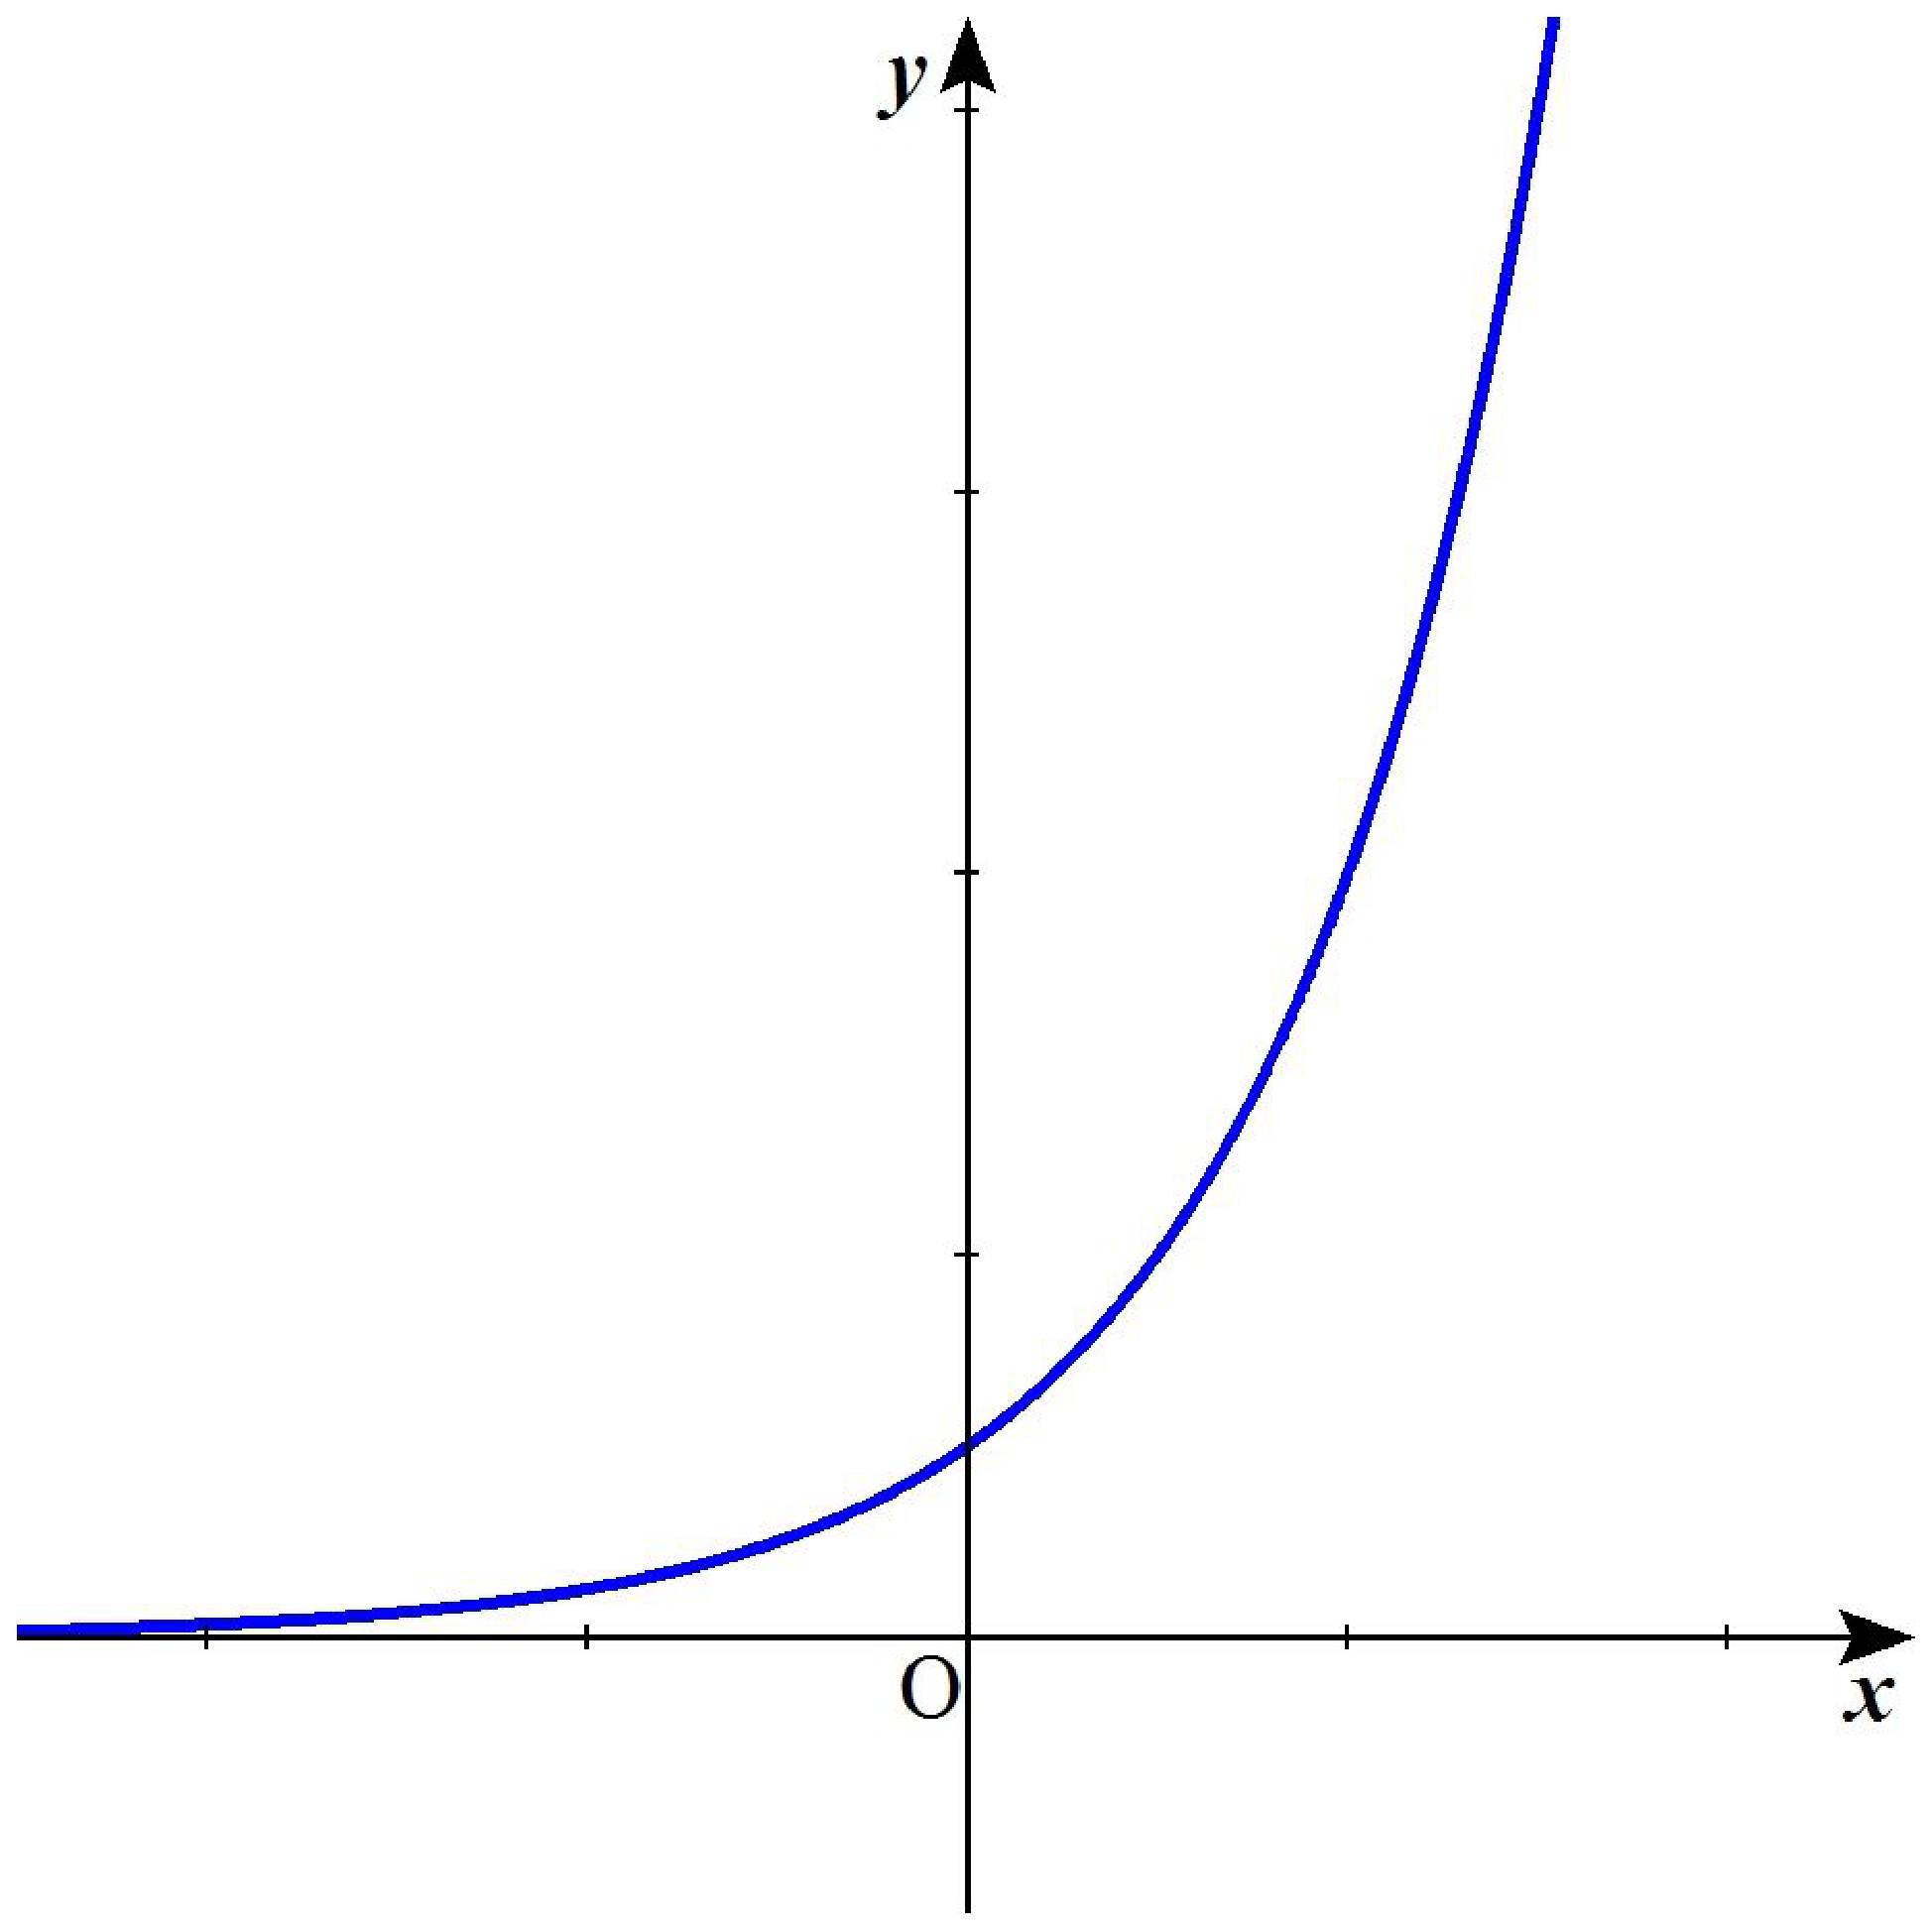
\includegraphics[width=8cm]{../figures/sisuu.eps}
  \caption{指数関数}
\end{figure}

こいつを, x軸方向に様々な点で接線ぽいのを引き, 傾きを推測してみてください. \\
\\
面白い事に, こうやって求めた傾きの値をy成分として新しくグラフを書いた f(x)' も指数関数の形をしているのです!!\\
\\
察しの悪い人用に言うと,限りなく負の方向に行ってるとほぼ横に伸びてるので,その接線の傾きもほとんど変化しませんね?一方で正の方向は逆に進めば進むほど傾きが急になります.傾きの変化を関数としたのが微分なんだから,これが元の関数と同じ形になるってのも不思議じゃない気がしてきましたね?\\
\\
そしてこの形は, (0,1)だけは固定としてその開き方が底の値によって異なります. \\
底の値次第で, 微分したら開いた指数関数がでてくるものや, 細くなった指数関数がでてくるのです.\\
\\
もう分かりますね?ネイピア数とは, 丁度この開いたり閉じたりする境界にある数なのです!!\\
よって微分しても出てくる指数関数は開き具合を変えず, 重なった関数となるのです.\\
\\
ネイピア数の何がすごいかって?\\
いろんな数学に利用できるところです!!!\\
\begin{eqnarray}
\mathrm{e}^{i\theta} = \cos\theta + i\sin\theta \\
F(x)=\frac{1}{\sqrt{2\pi \sigma^2}}\int_{-\infty}^{\infty}\exp{\left\{-\frac{(x-\mu)^2}{2\sigma^2}\right\}}\ \mathrm{d}x
\end{eqnarray}
書くのが面倒なのでいかついのは1個だけにします. ガウス関数ですね. 統計とか信号処理やるときにでてきます. 上は言わずもがなのオイラーの公式です.\\

\subsection{常微分と偏微分,全微分}
微分というと,大学以降とかで常微分だとか偏微分だとかといった言葉を聞いたことがある人もいるかと思います.ただでさえ微分とかよく分からないとか思っていたのにその中にも色々あるとか言われても普通に困りますよね.ここではそいつらについて紹介します.実は全然難しくないです.\\

はじめに,常微分とその他2つの違いについて説明します.その違いは簡単で,変数の数です.先程まで説明に使っていた微分はどれも,変数が1つ,$x$だけの微分でした.でしたよね?

変数が一つ関数の微分を常微分と言います.今までやってたのは常微分でした.

\begin{eqnarray}
f'(x) =\lim_{dx \rightarrow 0} \frac{f(x+dx) - f(x)}{dx}
\end{eqnarray}

次,偏微分と全微分は何かというと,そう.変数が2つ以上の関数の微分です.微分の定義は局所的な微小変化率を求める事でした.では変数が2つ以上の場合生じる問題が,どの変数についての微小変化率を見るのかという話です.

ということで,全ての変数について微分しましょうとするのが全微分,どれか一つを選んで微分するのが偏微分です.それぞれ見ていきましょう.まずは偏微分.\\

\begin{eqnarray}
\label{eq:partial}
\frac{\partial f}{\partial x} = \lim_{dx \rightarrow 0} \frac{f(x+dx, y) - f(x, y)}{dx}
\end{eqnarray}

常微分に対して,$f(x)$が$f(x,y)$になっているだけですね.その分,$x$も$y$も動いた点は$(x+dx, y+dy)$として定義されます.しかし偏微分はそのうち片方,ここでは$x$についてのみ変化量を見たかったので,$x$のみ$dx$が足され,つまり移動し,$y$は固定されたままになっています.これを$x$の変化に対する$f(x,y)$の変化,$x$についての偏微分と言います.yについては勿論以下の通り

\begin{eqnarray}
\frac{\partial f}{\partial y} = \lim_{dy \rightarrow 0} \frac{f(x, y+dy) - f(x, y)}{dy}
\end{eqnarray}

3変数以上でもやり方は変わりません.

\begin{eqnarray}
\frac{\partial}{\partial x}f(x,y,z) = \lim_{dx \rightarrow 0} \frac{f(x+dx, y,z) - f(x, y,z)}{dx}
\end{eqnarray}

計算上は,結局のところ偏微分する変数以外は定数扱いするだけです.なのでたとえば

\begin{align}
f(x,y) = x^3 + 2y^2\\
\frac{\partial f}{\partial x} &= \lim_{dx \rightarrow 0} \frac{\{(x+dx)^3 + 2y^2\} - (x^3 + 2y^2)}{dx}\\
&= 3x^2
\end{align}

となります.$y$について偏微分すると$4y$ですね.
\begin{align}
df &= f(x+dx, y+dy) - f(x,y)\\
&= 
\end{align}

簡単ですね.さらに,偏微分が分かれば全微分も簡単です.早速定義していきます.

\begin{align}
\label{eq:all-partial}
y = f(x,y) \nonumber \\
df &= f(x+dx, y+dy) - f(x,y)\\ 
&= \frac{\partial f}{\partial x}dx + \frac{\partial f}{\partial y}dy
\end{align}

となります.

解釈しましょう.まず$f(x+dx, y+dy)$への変化なのだから,関数そのものの変化率を見たいわけですね.関数そのものの変化量になるので,$\partial$なんかは使わずシンプルに$df$となります.で,その計算が全ての変数についての偏微分に$dx, dy...$をかけたものを足し合わせで表せるよって事ですね.何故でしょう?\\


直観的に,偏微分足すのは良いでしょうか.x,yそれぞれの方向に対する変化量を足せば両方を移動させた事になるよねって話です.では何故$dx, dy$をかけるのかですが,ここで偏微分が何をするものだったか思い出しましょう.その変数方向での変化率,傾きを出すんでしたね.傾きaの直線でb移動したところの点,と考えれば分かるでしょうか.単純にab移動するんでしたね.全微分の場合,ずらすのはそれぞれ$dx, dy$なので,傾き(偏微分)に移動距離$(dx,dy)$をかける事で移動量を出せるというわけです.

そいつらを足し合わせれば,正味の移動量が分かるよね,というのが全微分でした.まとめ!

\begin{screen}
微分
\begin{eqnarray}
f'(x) =\lim_{dx \rightarrow 0} \frac{f(x+dx) - f(x)}{dx} \qquad \text{常微分} \nonumber \\
\frac{\partial f}{\partial x} = \lim_{dx \rightarrow 0} \frac{f(x+dx, y) - f(x, y)}{dx} \qquad \text{偏微分}\nonumber \\
df = \frac{\partial f}{\partial x}dx + \frac{\partial f}{\partial y}dy \qquad \text{全微分} \nonumber
\end{eqnarray}
\end{screen}



\section{積分}
さて, 微分がわかったとこで積分の気持ちです. パパっといきます.\\
まず, 計算の上でいえる事としては, 微分の逆の操作をするという事です.
\begin{eqnarray}
\label{eq:int}
\int 2x dx= x^2 + C
\end{eqnarray}
こんな具合でしたね. \\


\begin{lstlisting}[caption=\ref{eq:int}のコード,label=sc:int]
int(2*x)
\end{lstlisting}


微分とは微小な増分であるdxとdyを用いて変化率を求めるものでしたが, 積分の場合は, dxとyを用いて面積を求める操作になります.\\
\\
関数f(x)は x = a の時, f(a)という値を取り, x = b の時, f(b)という値を取ります. この時xの増分 dx は, x軸での距離を表すので横の長さととらえる事ができ, f(a)あるいはf(b)は縦の長さと考える事ができます.\\
\\
こうして定義される横と縦を用いて作られる長方形を, a~b, b~c, c~d..., m~nといった範囲で同じように作っていき, それぞれの面積をたすと, 関数f(x)とx軸の間の, a~nにおける面積っぽいものがだせますね!\\
しかしこのとき, 横はまだしも縦の長さが問題です. 左端に合わせるのか右端に合わせるのか, あるいはその中点にするのか... これによって求められる面積は理論値から離れた値になってしまいます.\\
\\
この問題を解決するにはどうしたらよいでしょうか?\\
簡単ですね, x軸上での幅を限りなく小さくしていけばよいのです!!\\
\\
横幅が限りなく0に近づいた時, 左端と右端のとる高さは同じ値となるため, 微小長方形の形も関数f(x)にそったものになるはずです.\\
\\
そしてそれらを足し合わせれば, デコボコではなく滑らかな, 関数f(x)の凹凸にあった面積を導出する事が出来るのです!!!
\begin{eqnarray}
\label{eq:int2}
\int_a^b f(x) dx
\end{eqnarray}
とはつまり...\\
xがaからbの範囲において, それぞれの f(x) = 高さと 微小なdx = 幅をかけたもの = 面積を足し合わせる\\
といった意味になっているのです!!!



\begin{lstlisting}[caption=\ref{eq:int2}のコード,label=sc:int2]
int(fx, [a b])
\end{lstlisting}


\begin{figure}[H]
\label{im:integral}
  \centering
  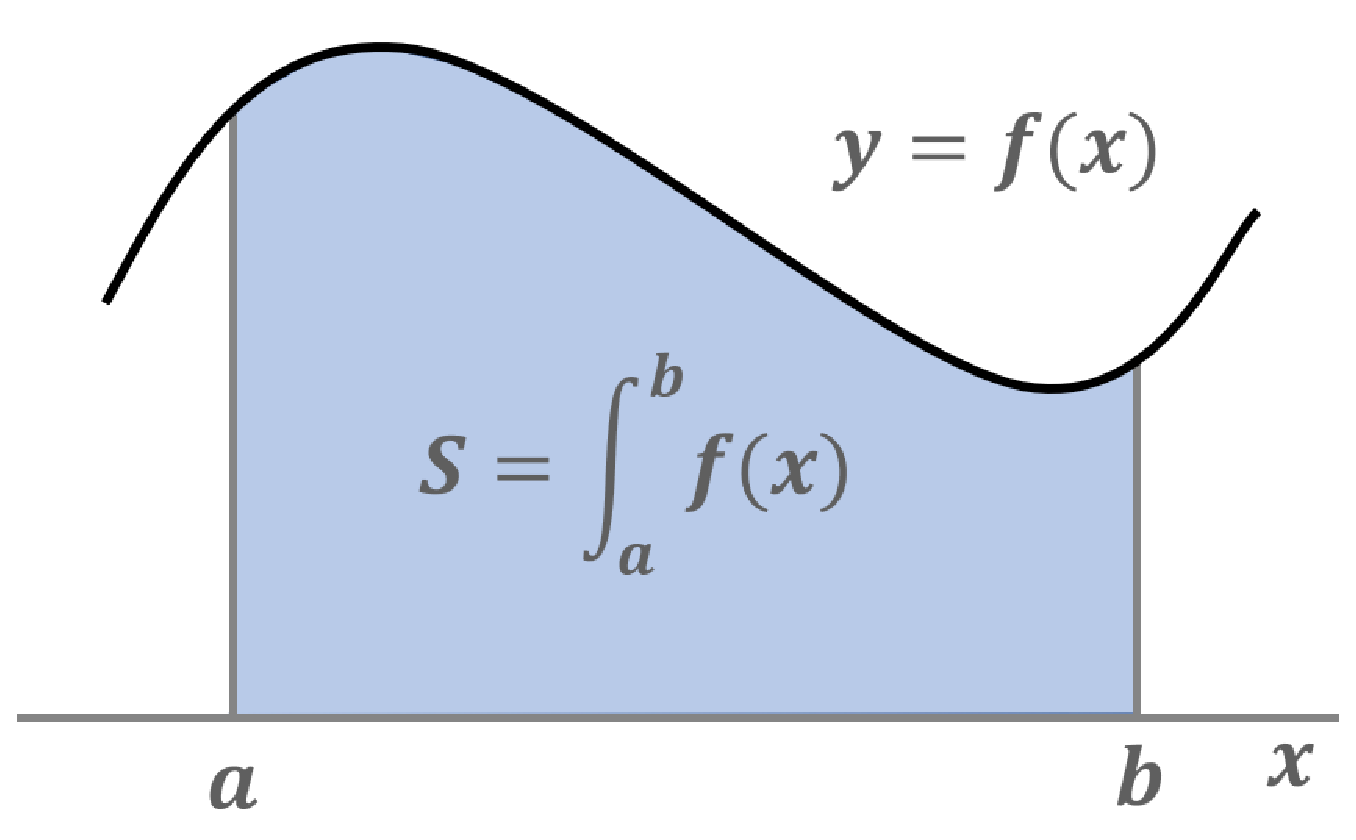
\includegraphics[width=10cm]{../figures/int.eps}
  \caption{積分と面積の関係}
\end{figure}


\subsection{足し算としての積分}
積分とは微小面積の足し合わせと言いましたが, 足し算はΣで表されたはずです. 何故∫を使うのでしょうか?\\
\\
答え. Σは離散値の計算にしか使えないからです!\\



\begin{eqnarray}
\label{eq:sum2}
\sum_{k=1}^{n} k
\end{eqnarray}

\begin{lstlisting}[caption=\ref{eq:sum2}のコード,label=sc:sum,  keepspaces=true]
K = [k1 k2 k3 ... kn]    // 数列の定義.実際は数字とか好きなのいれてください.
sum(K)
\end{lstlisting}


この式(\ref{eq:sum2}), コード(\ref{sc:sum})では, kに入る数字は1からnまでの整数になります. 無限小の幅による微小面積を考えるときにこれでは, 全く意味がないですよね.\\
\\
そこで∫を使うと, 整数に限らずすべての数を足し合わせる事が出来るのです!!\\
素晴らしいですね!!!足し算のアップデートです!!!\\
\\
足し算として積分を使うことは, ここからの数学では, 頻繁に出てくるので是非感覚として理解してください.
\begin{eqnarray}
\label{eq:int3}
X(\omega) &=& \mathcal{F}[x(t)] = \int^{\infty}_{-\infty}x(t)\exp(-j \omega t)dt \\
 x(t) &=& \mathcal{F}^{-1}[X(\omega)] = \int^{\infty}_{-\infty}X(f)\exp(j \omega t)dt 
\end{eqnarray}
たとえばこいつらは複素フーリエ変換とその逆変換の式ですが, これらもx(t)とexpなんたらの掛け算の-∞から∞での総和とかのように解釈する事ができるわけです!!!\\
とは言っても,実際PCに計算させる時には計算を楽にさせるためだったり,そもそも計測されたデータが離散だったりするために積分でなく足し算だったりしますが...\\

足し算の拡張として積分が扱えるようになったところで, その応用法について考えます. 
\subsection{関数の内積 \label{dot_func}}
\ref{dot}では, 関数の内積を定義する際にΣの代わりに∫を使いました. その理由は, 上記の通り積分を使う事で, Σでは表現できなかった非整数も演算に組み込む事が出来るからです.\\
\\

\begin{eqnarray}
\label{eq:dot_func}
z = \int^{\infty}_{-\infty} f(x)g(x)dx
\end{eqnarray}

式(\ref{eq:dot_func})が関数の内積の定義です. 日本語では, 同じ点xについての関数f(x),g(x)それぞれの値を算出し積を計算し, それをすべて足し合わせるという意味です. 当然, 直交していれば0の値を取るのは変わりません.


\subsection{畳み込み積分 \label{convolution}}
お次はいよいよ, ウェーブレットやヒルベルトを勉強する上でも必須になる, 畳み込み積分について学びます.\\
先に定義式を置いておきます.

\begin{eqnarray}
\label{eq:convolution}
f(t) , g(t)\\
h(t) = \int^{\infty}_{-\infty} f(\tau) g(t - \tau) d\tau
\end{eqnarray}
式(\ref{eq:convolution})から読み取れる事ですが, まず同じ変数(ここでは時間t)に対する関数である, f(t) , g(t)が定義されています. こいつらの式は任意ですが, 同じ変数に対応している事は重要です. \\
次に, 計算結果として求められるのも関数になっていますね. 計算結果であるh(t)の引数も, f(t)g(t)同様にtですね.\\
そして最後に, 右辺では関数fの引数は$(\tau)$となっていて, gの引数も$(t - \tau)$となっていますね. ここが内積と異なる点です. また, それぞれの関数の引数を足し合わせる事で常に一定の値を取る事も分かります $(\tau + t - \tau = t)$\\
\\
tを時間とした場合でこの式を説明すると, $\tau$は定義域の中のある瞬間の時間を指します. よって$f(\tau)$は「ある時間$\tau$におけるf(t)の値」ですね.\\
という事は$g(t-\tau)$は, 時刻t(つまり現在)から, ある時刻(関数fによる作用が起きた時)までの時間差を指します. それらの積を $\tau$で積分するというのがこの式の意味ですね.\\
\\
\\

陰キャの皆さんは, いつも悲しい事ばかり経験している事と思います. 本書に載ってるレベルの数学も理解できない絶望感, 何故か自分だけ新歓されない孤独感, 笑顔で挨拶してくれたから脈ありかなと思った女の子に告ったらブロックされた無力感...\\
\\
可哀想に. 僕みたいにイケメンの陽キャと違って, 陰キャの皆さんは人生ハードモードですね.\\
\\
ですが大丈夫です. どんな心の痛みも, 数日寝てゲームして数学してれば
.........まぁ, 時間が解決してくれるはずです. \\
\\
さて, 人生を時間軸とすると, 陰キャの暗く惨めでむごたらしい人生では絶え間なく心に傷を負う「イベント」が起きるはずです. このイベントで受ける心の傷の大きさは場合によりけりなので, 時間依存の変数, つまり時間関数と捉えられます\\
(このたとえだと普通はとびとびの離散値になりますが, 究極の陰キャを想定して連続値を取る関数にしておきましょうか. 頑張れ陰キャ, 負けるな陰キャ. 君には数学がついている)\\
\\
つまり, 関数f(t)ですね!!\\
\\
しかし先程も言ったように, 普通は心の傷は時間経過で減少していきます. ここで, その減少の仕方を関数g(t)としましょうか. こいつも同じく時間関数ですよね.\\
勿論, 中には1年くらいしてから心の傷がぶり返す面倒なオタクもいますので, 関数g(t)の形はなんでもいいです.\\
\\
ここで, とある瞬間$(\tau)$に陰キャが自分だけクラス会に呼ばれなかった時に受けた心の傷を$f(\tau)$とおきます.\\
今日は時間tの時点です. つまり陰キャが心に傷を負ってから$(t-\tau)$日が経過しているわけですね. 傷が癒えるのは時間依存の関数g(t)によりますから, 今日陰キャ君が感じている, クラス会による心のダメージ h(t) は
\begin{eqnarray}
\label{eq:inkya_otu}
h(t) = f(\tau) g(t-\tau)
\end{eqnarray}
で表せますね!!式(\ref{eq:convolution})に近づいてきました. \\
改めて, 式(\ref{eq:convolution})を確認してみます.
\begin{eqnarray}
h(t) = \int^{\infty}_{-\infty} f(\tau) g(t - \tau) d\tau
\end{eqnarray}

式(\ref{eq:inkya_otu})を$-\infty$から$\infty$の範囲で, 時間$\tau$について積分したものがh(t)になっていますね.\\
積分が何をする操作だったのかを考えれば, この式の残酷さが分かるはずです.\\
関数 f(x) について, 範囲aからbまでをxで積分というのはつまり...\\
「xがaからbの範囲の全ての数を取った時のf(x)の値を足し算する」事でした. \\
\\
上記の陰キャの例で考えるなら, 式(\ref{eq:convolution})は「時刻tの時, 陰キャ君が感じている苦痛($-\infty$から$\infty$の間に受けた心の傷の足し算)」です.\\
\\
時刻$\tau_1$の時にクラス会からハブられた$f(\tau_1)$も...\\
時刻$\tau_2$の時に可愛い女の子にLINEのスクショをTwitterに晒された$f(\tau_2)$も...\\
時刻$\tau_3$の時に洗車したての車のフロントに鳥の糞が落ちた$f(\tau_3)$も...\\
時刻$\tau_4$で未保存のtexファイルを誤って閉じちゃった$f(\tau_4)$も...\\
\\
その全てを足し算したものがh(t)なわけです. ここでtは現在の時刻です. \\
$g(t-\tau)$によってダメージは小さくなってるので, 実際は$\tau_4$のダメージは計り知れず, $\tau_1$のダメージはそれほどではないかもしれませんが, とりあえずそういう事です. \\
\\
h(t)には陰キャくんの辛く惨めで凄惨な人生が詰まっているのです!!\\
......おい待て,早まるな.h(t)は時間関数だ.今はつらくてもいつか楽になれるさ.頑張れ.



\subsection{つまり畳み込みとは}
さて, 皆の心を犠牲にして流れを理解できたところで, 最後に数学的な言葉で畳み込みの確認をします.

\begin{eqnarray}
\label{eq:conv}
h(t) = \int^{\infty}_{-\infty} f(\tau) g(t - \tau) d\tau
\end{eqnarray}

式(\ref{eq:conv})は, 「全ての瞬間($\tau$)に入力(関数f)されたそれぞれの信号が,処理システム(関数g)によって変換されていて, その総和が現在出力されている信号h(t)である」を意味します. これを各時間について計算したものが関数h(t)なので...\\
\\
畳み込みとは, 「関数fが関数gによって変化させられた関数hを求める処理」というわけですね!!!\\
脳波の話をするなら, band-pass-filterとかを考えてみて下さい. 生データが, フィルターをかける事で特定周波数帯域のみの信号に変換されますね. \\
\\
信号処理の話を理解するためには, 畳み込みはかかせない概念です. かなり丁寧に説明したので, 頑張って理解してください.\\
\\
余談ですが, 畳み込みは可換なので, 以下は同じことを指す式です.注意.

\begin{eqnarray}
h(t) = \int^{\infty}_{-\infty} f(\tau) g(t - \tau) d\tau=
 \int^{\infty}_{-\infty} f(t-\tau) g(\tau) d\tau
\end{eqnarray}

\begin{figure}[H]
\label{im:convolution}
  \centering
  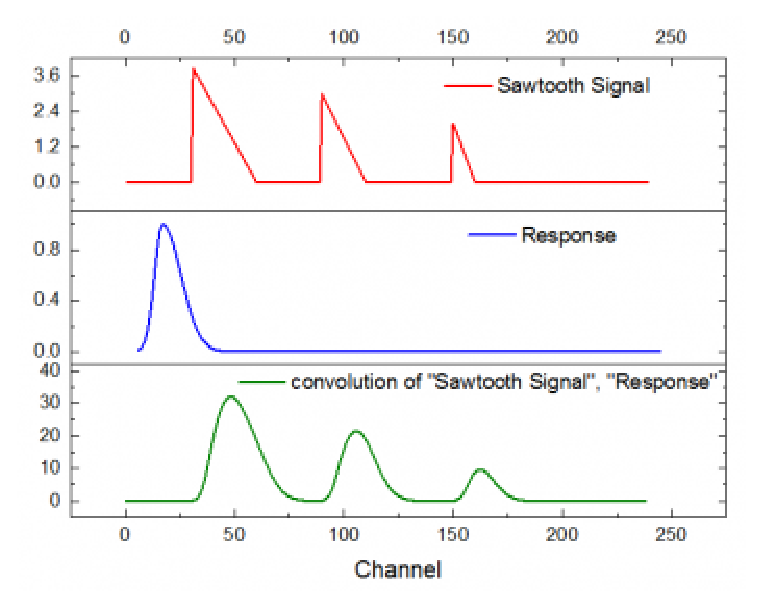
\includegraphics[width=10cm]{../figures/Convolution.eps}
  \caption{畳み込みのイメージ (OriginLabより)}
\end{figure}

\begin{lstlisting}[caption=畳み込みのコード,label=sc:conv]
x = cos(3 * [0:0.1:20]);
y = [zeros(1,100) ones(1,20) zeros(1,81)];
z = conv(x,y);

subplot(2,1,1);
plot(x)
hold on
plot(y)

xlim([0 200])
ylim([-1.2 1.2])
legend('三角波', 'フィルター')
title('Raw signal and filter')
hold off

subplot(2,1,2); 
plot(z)
xlim([0 400])
title('Filterd signal')
\end{lstlisting}

\begin{figure}[H]
\label{im:conv2}
  \centering
  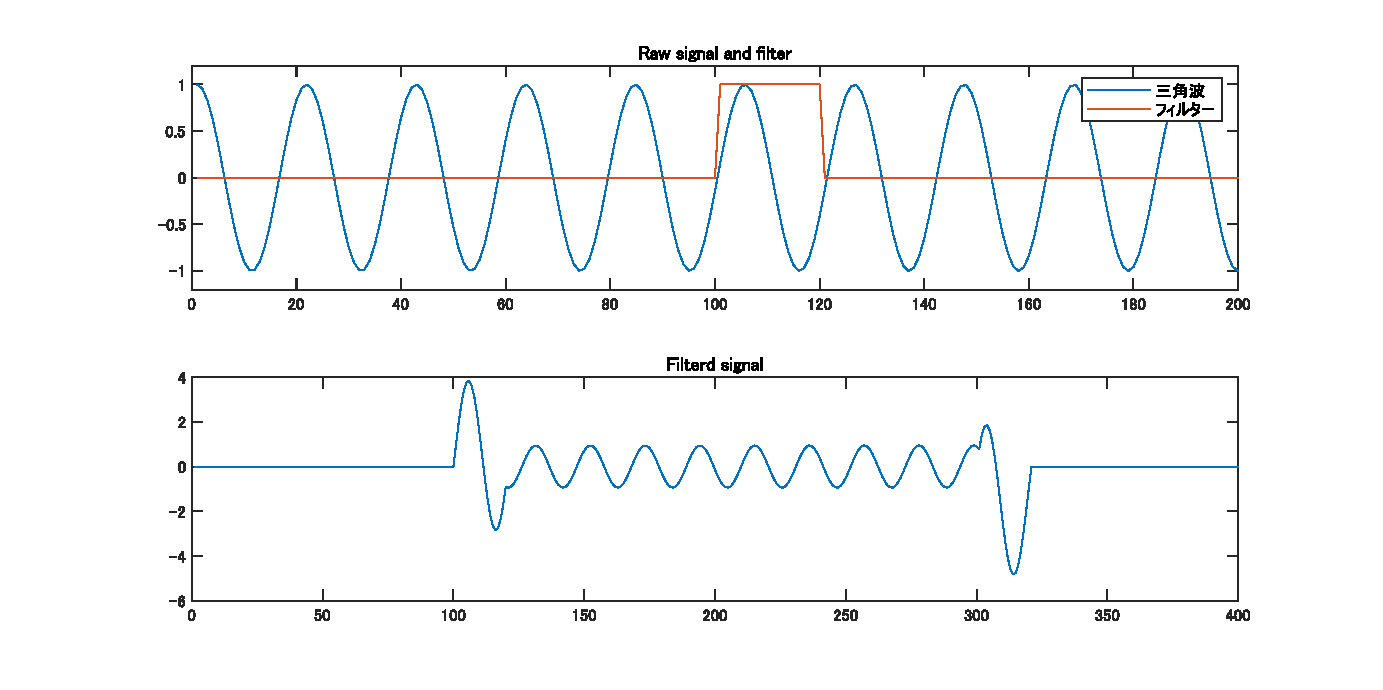
\includegraphics[width=10cm]{../figures/conv.eps}
  \caption{コード(\ref{sc:conv})の図}
\end{figure}

上にあげたコードによって計算された結果が図(\ref{im:conv2})になります.いくつか気づく事があると思います.まず青の三角関数は0から100までの間0を保つように変形されましたね.同じくお尻の方もなっています.こんな使い方をするのがフィルターです!\\
今回は時間方向でそのままやっていますが,これを例えば一度周波数変換した信号に対しかけて,もう一度元の時間関数に戻す作業をしてあげれば,ここでいうオレンジのフィルターにかかっていた周波数帯域だけが元に戻ることになります.そう,周波数フィルターですね!!!\\
\\
他にも気付くことがありますね,まずフィルタの長さよりも変形された信号の方が長くなります.これは畳み込みの計算上仕方ないですね.重なっている部分の積の和をとるわけですから.\\
そしてこれによって生じるもう一つの問題,それが畳みこまれた信号の両端に生じている謎の突起です.\\
これも計算を考えれば道理ですが,フィルタの一部だけが信号にひっかかっている状態だとすべての要素の積が計算されるわけではありません(正確には0との積が行われている).つまり本来であれば積の結果が負になったりするはずの部分が計算されていないわけですね!これが原因で,フィルタが信号に全部かかるまでの範囲は計算結果が一寸おかしな挙動をします.\\
これはanalysisとかでいずれやると思いますが,畳み込みの際に気を付けないといけない事で,edge artifactなんて呼ばれていたりするものです.心の片隅においておいてください.


\chapter{統計学}
\section{基本統計量}
この節では統計の基礎を学びます. 統計は脳波解析に直接的に使うわけではありませんが, 解析した結果がいいデータなのかゴミデータなのかを判断したりするために必要です. また, 分野問わずどんな論文も統計の知識なくては読むことが出来ません. 幾何学などに比べれば大した事ない量とレベルなので, パパっと身に着けちゃいましょう!! (脳にフィットするとは言っていない)\\
\\
さて, まずは冗談じゃなく小学生でも知ってる統計学から始めましょう.\\

はじめに,アンケートである学校の男子1000人の平均身長を聞いてみたとしましょうか.
\begin{figure}[H]
\label{im:histgram}
  \centering
  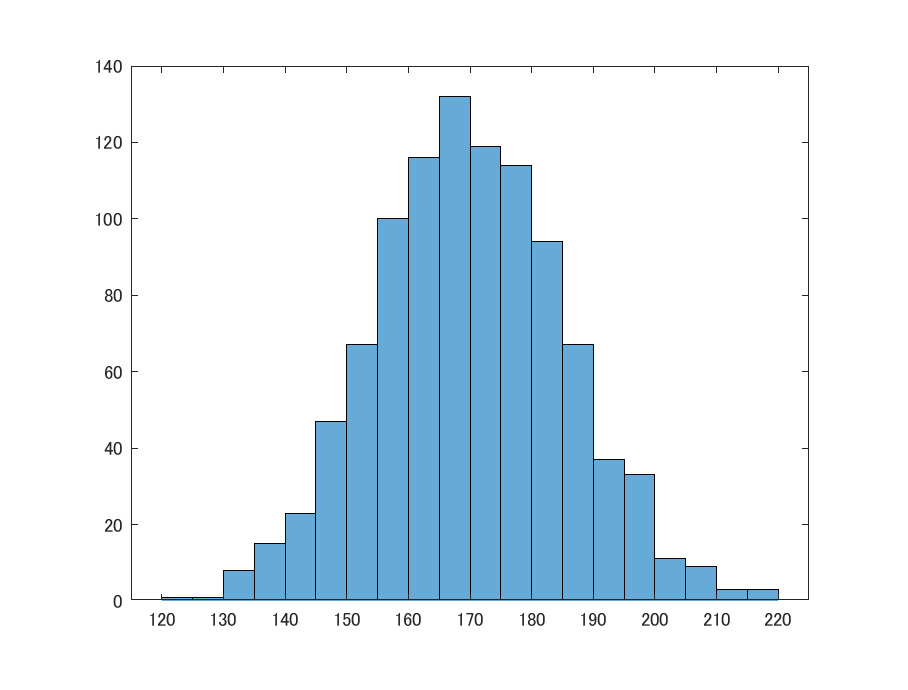
\includegraphics[width=10cm]{../figures/hist.eps}
  \caption{アンケートした架空の男子高校生の身長(平均170, 標準偏差15)}
\end{figure}

複数の数値データ$x_i = [x_1, x_2, x_3, ...]$が得られた際, とりあえず平均と分散, ついで標準偏差を求めたくなるのは人間の性ですね.\\

\begin{screen}
基本統計量
\begin{eqnarray}
\label{eq:ave}
\bar{x} = \frac{\sum_{i=1}^{n} x_i}{n}  \qquad \text{平均}\\
\label{eq:var}
s^2 = \frac{\sum_{i=1}^{n} (x_i - \bar{x})^2}{n} \qquad \text{分散}\\
\label{eq:dev}
s = \sqrt{s^2} = \sqrt{\frac{\sum_{i=1}^{n} (x_i - \bar{x})^2}{n}} \qquad \text{標準偏差}
\end{eqnarray}
\end{screen}

\begin{lstlisting}[caption=式(\ref{eq:ave}\ref{eq:var}\ref{eq:dev})のコード,label=stat]
x = [1 2 3 4]
mean(x)
var(x)
std(x)
\end{lstlisting}


とりあえず, 平均(\ref{eq:ave})と分散(\ref{eq:var}), 標準偏差(\ref{eq:dev})の式を書いてみました. 平均は良いですね?全要素を足して要素数で割るだけです.\\
分散は, 一見ややこしくなってるかもしれませんが各要素と平均の差(偏差)を足して, 同じく要素数で割っています. 標準偏差はその平方根です.\\
\\
 平均とは, 得られたデータのだいたい「真ん中あたり」を指す指標です. 代表値として, 他には中央値とか最頻値とかがいますが, まあ平均値だけ覚えていれば大丈夫です. モブは放置.\\
\\
 分散とは, 偏差の平均的な奴ですね?つまり, 得られたデータはどれだけ平均付近に固まっているか, あるいはバラバラになっているかを指します. 各要素が平均から遠い値であるほど, 偏差とその二乗は大きな値を取ります. 2乗するのは, 符号の影響をなくすためです. そいつらの平均なので, やはり値が大きい程データがばらついているという事になります.\\
\\
 標準偏差は, 分散の平方根です. それだけ. 偏差の特性上, 分散を導出する際にデータを2乗してしまっているため, 分散は元のデータとスケールが違います. 例えば元データが長さだったら, 分散は面積を表してしまいます. なので平方根をとって次元をそろえてあげるわけですね. これで分かりやすくなります.\\
\\
 図(\ref{im:histgram})に設定した統計量とヒストグラムを見比べて, 感覚を確認してください.
\\
 こいつらは後程アップデートされたりしますが, 基本的にはデータを扱う上で普遍的に利用されるものです. まず確実に理解しておきましょう.\\
\\

\subsection{正規化}
ちなみに, 標準偏差と平均をどう使ってデータを読み解くのかという例として, こんなのもあります.

\begin{eqnarray}
\label{eq:normalize}
z_i = \frac{x_i - \bar{x}}{s}
\end{eqnarray}



\begin{lstlisting}[caption=式(\ref{eq:normalize})のコード,label=sc:normalize,  keepspaces=true]
x = [1 2 3 4]
for i=x
    z([i]) = ((x([i]) - mean(x)) / std(x))
end
z = normalize(x)        // 関数使うとこう
\end{lstlisting}



正規化(標準化)と言われる処理です. 各要素と平均との偏差を標準偏差で割っていますね. 標準偏差はざっくり言うなら偏差の平均的なやつですので, それと各偏差の比を見ているわけです. こうする事で, 平均0, 分散1のデータに置き換える事が出来るので, それぞれの要素がどれくらい平均から外れているかが分かりやすくなります. zの大きさが1を超えれば平均からかなり(正なら正方向, 負なら負方向に)離れているってわけですね!!\\

\begin{figure}[H]
\label{im:z-hist}
  \centering
  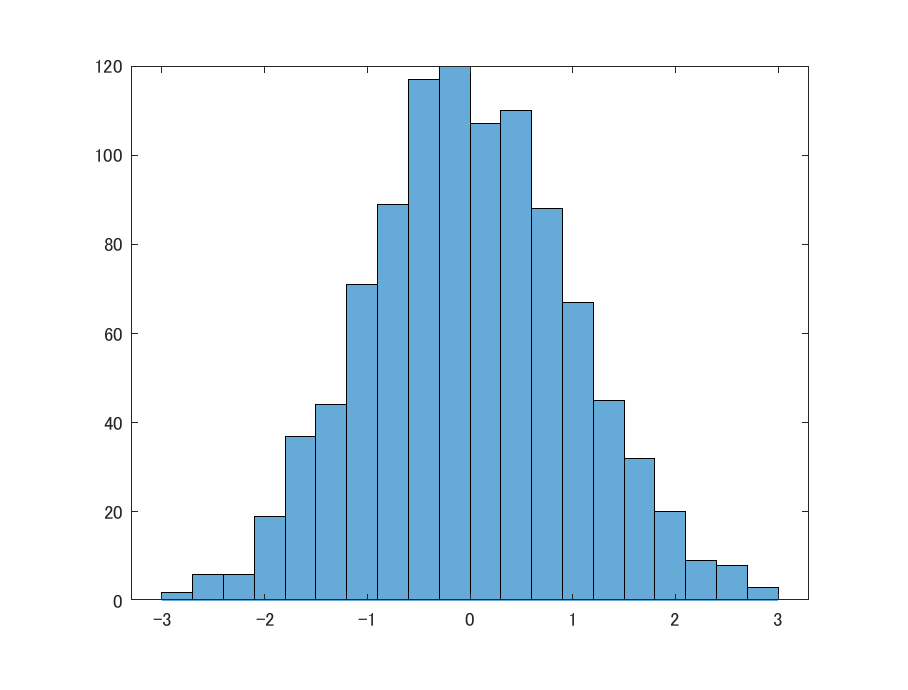
\includegraphics[width=10cm]{../figures/z-hist.eps}
  \caption{正規化した, 同じ条件の図(\ref{im:histgram})}
\end{figure}

まぁ, 勿論こんな事しないでそのまま眺めるだけでも十分だったりしますが.

\section{相関と共分散}
次もよくつかわれる基礎です. 2つ以上の変数を持つデータ(たとえばAさん,Bさん ... の身長と体重)の性質を検証する術です. \\
\subsection{相関と散布図}
相関は非常に簡単です. 
\begin{lstlisting}[caption=図(\ref{im:scatter})のコード,label=sc:scatter]
// 正の相関あり
x = [0:0.1:10]+ rand(1,101)
y = [0:0.1:10]
scatter(x,y)

// 負の相関あり
x = [0:0.1:10] + rand(1,101)
y = [0:-0.1:-10]
scatter(x,y)

// 相関なし
x = rand(1,100)
y = rand(1,100)
scatter(x,y)
\end{lstlisting}

直交座標軸横軸に変数1, 縦軸に変数2をおいて, あとは得られたデータをすべて対応する位置にデータを点でプロットしていくだけです. こうして得られた, 点を散りばめられた図を散布図だとか相関図と言います.\\
 この図の特徴ですが, データによって点の散らばり方が変わります. たとえば先程の身長と体重の例の場合, 一般的に身長が高い人の方が体重が重い傾向にありますね?これは図では点が右肩上がりの斜めライン付近に多く集まる事を意味します. \\
 逆に, 右肩上がりの斜めに点が集まるという事は, 一方が上がると他方も上がる, 比例に似た関係にあると言えます. 逆に右肩下がりの場合, 一方が上がると他方が下がる関係ですね!!\\

\begin{figure}[H]
\label{im:scatter}
  \centering
  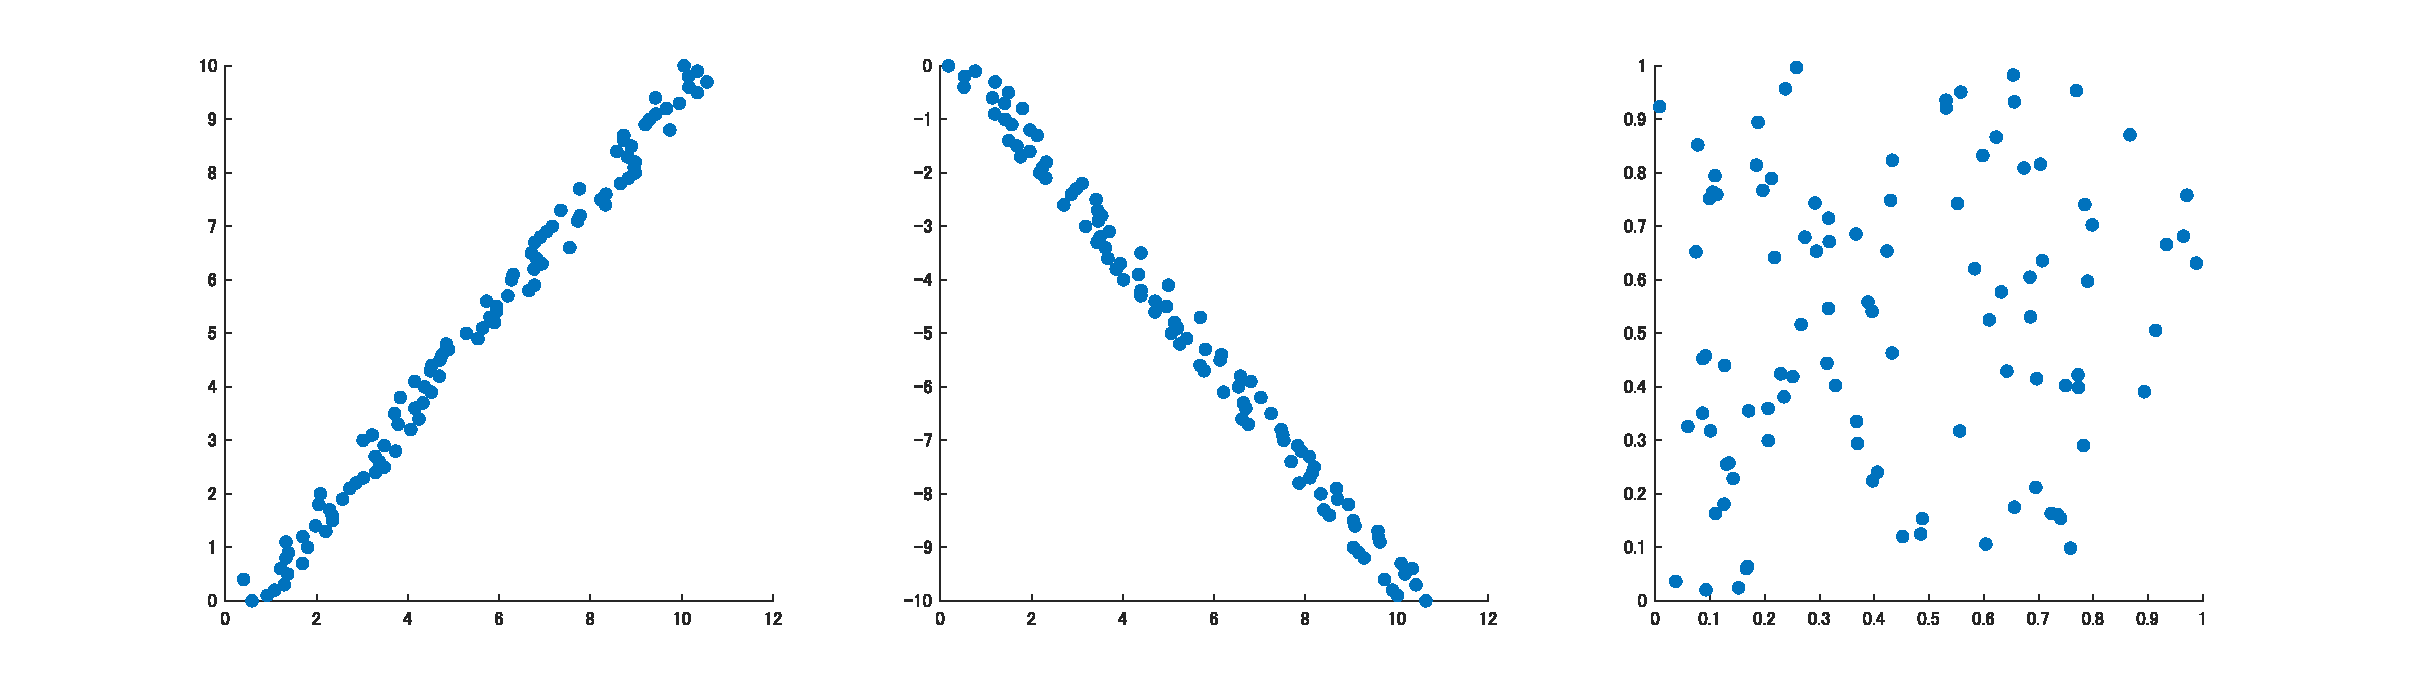
\includegraphics[width=15cm]{../figures/scatter.eps}
  \caption{左: 正の相関図 中: 負の相関図 右: 相関なし}
\end{figure}

前者を正の相関, 後者を負の相関があるといいます.散布図を描いた時の見た目でなんとなくデータ間の関係が分かるわけです. 見た目ではっきり分かるほど点が線状に並ぶ程, 相関が強いと表現されます(図\ref{im:scatter}左, 中はかなり強い). 逆に見た目で何も分からん場合(図\ref{im:scatter}右)は, データ間には相関がないと言えます. \\
 非常に便利なので, アンケートデータとか取ったらとりあえずプロットしてみると良いです. 
\\
\subsection{回帰}
相関は2つの変数の間に区別を設けず,対等に見て関係を見る方法でしたが,それに対して片方を使ってもう一方を見るのを回帰といいます.つまり変数$\mathbf{x}$によって変数$\mathbf{y}$が決定される様子を表すものです.\\
 一般に,たとえば身長と体重などどっちがどっちの原因であるとかは考えにくいものに対しては使いませんが,人口とGDPみたいに, どちらかがどちらかの原因になっているかが分かるようなデータに対して使うと,実際どの程度依存しているのかを計算できるものです.この場合,人口が独立変数,GDPが従属変数となります.では回帰ですが,ここでは一番簡単な線形回帰,単回帰分析だけ触れてみましょう.\\

 単回帰分析は,独立変数をx,従属変数をy軸において散布図を作った際に一番 ``それっぽい'' ところに直線を引く手法です.小学校とかの理科の実験レポートでやりましたね.あれです.

 そう, 近年では意識スカイツリー系イケイケ起業マンたちに「AI」と呼ばれていたりもする,あれです.散布図が描けて, あとは最小二乗法(図\ref{im:predict})が使えちゃえばAIエンジニアが名乗れるのです.素晴らしい時代ですね.嘘です.とかく,まずはPCにやってもらった結果を見てみましょう.\\


\begin{figure}[H]
\label{im:predict}
  \centering
  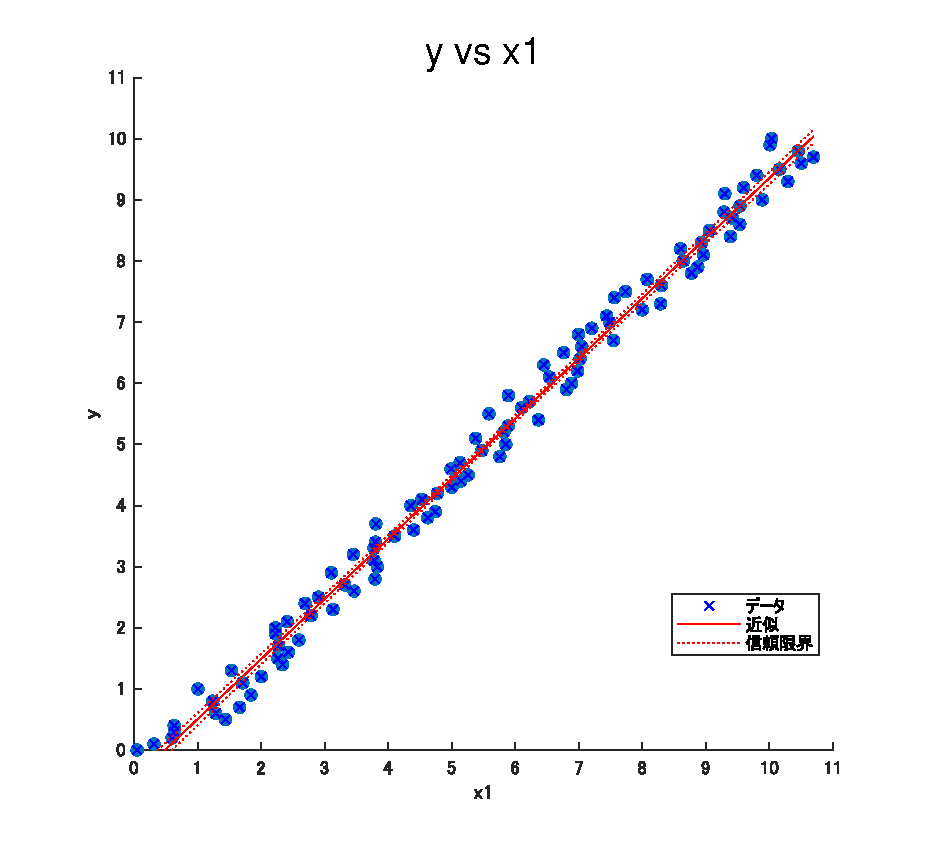
\includegraphics[width=8cm]{../figures/predict.eps}
  \caption{AIエンジニアわい迫真の単回帰分析}
\end{figure}


\begin{lstlisting}[caption=単回帰のコード,label=sc:regression]
x = [0:0.1:10]+ rand(1,101)
y = [0:0.1:10]
mdl = fitlm(x,y)
scatter(x,y)
hold on
plot(mdl)
hold off
\end{lstlisting}

良い感じですね.たしかにそれっぽいところに線が引かれています.でもMATLABのこのコード使い方がいまいち分からなかったのでtitleとかいじれなくてモヤモヤしてます... \\

では次に,PCが何をやったのか自分たちで数学をやってみましょう.先程一瞬でてきた最小二乗法とは,予測値$\hat y_i$と実測値$y_i$の差の全データでの二乗和を最小化する方法を意味し,今回の場合に利用すると以下の計算になります.

\begin{eqnarray}
\argmin_{a,b} L = \sum_{i=1}^n \{ y_i - (bx_i + a) \}^2
\end{eqnarray}

$\argmin_{a,b} L$は,関数Lが最小値を取るような変数a,bの集合という意味で,つまりここでは二乗和(L)を最小化するようなa,bの組み合わせを探すという意味です.実際のyの値と,直線すなわちxの一次関数で表してみた予測値との誤差を全てのデータについて足し合わせたものが二乗和です.二乗しているのは符号の影響を打ち消すためです.

 この二乗和が小さいということは,予測値と実測値のずれが小さいという事になりますね?それを計算するわけです.計算方法はそれぞれ最小値を取るわけですから,偏微分しましょう.すると

\begin{eqnarray}
\frac{\partial L}{\partial a} = \sum y_i -(\sum x_i)b + \sum a \\
\frac{\partial L}{\partial b} = \sum x_i y_i - (\sum x_i)a- (\sum x_i^2)b
\end{eqnarray}

が出てきます.これを正規方程式なんて呼んだりもするそうですが,とりあえずこいつらが同時になりたてば良いわけなので連立方程式として解きます.すると

\begin{eqnarray}
a = \bar y - b\bar x\\
b = \frac{\sum x_i y_i - n \bar{x} \bar{y}}{\sum x_i^2 - n\bar{x}^2}
\end{eqnarray}

と,a,bの値を求める事が出来ます.あとはこのパラメータに従った直線を引けば(図\ref{im:predict})のような事が出来るわけですね.なおここで,$\sum a = na, \bar x = \sum x_i/n, \bar y = \sum y_i/n$を用いてます.

\subsection{共分散}
変数間の関係を探るのに非常に便利な相関ですが, やや客観性にかけていた事に気付くでしょう. 「なんとなく」「それっぽい」などの語彙を多用していたはずです. これでは困ってしまいますので, より客観的に評価する方法を考えます.\\
\\
 それが共分散というやつで, 普通の分散は1変数において偏差の二乗平均を取るわけですが, 共分散では2変数の偏差同士を掛け合わせます. こうする事で, それぞれの偏差の特徴を反映させた新しい分散を定義する事が出来ます. \\
\\
 それぞれの特徴とは, 偏差の符号です. 1変数分散の場合は単に二乗してしまうため符号は外れますが, 共分散の場合はそれぞれの偏差の符号が異なった場合には負の値を取ります. 偏差の符号が異なるというのは負の相関が, 同じなら正の相関があるという事です.\\
さらに, 絶対値の方も有用な情報をくれます. それぞれの偏差が大きい程, 共分散の絶対値も大きくなるわけです. これは相関の強さを表します.\\

\begin{figure}[H]
\label{im:co-var}
  \centering
  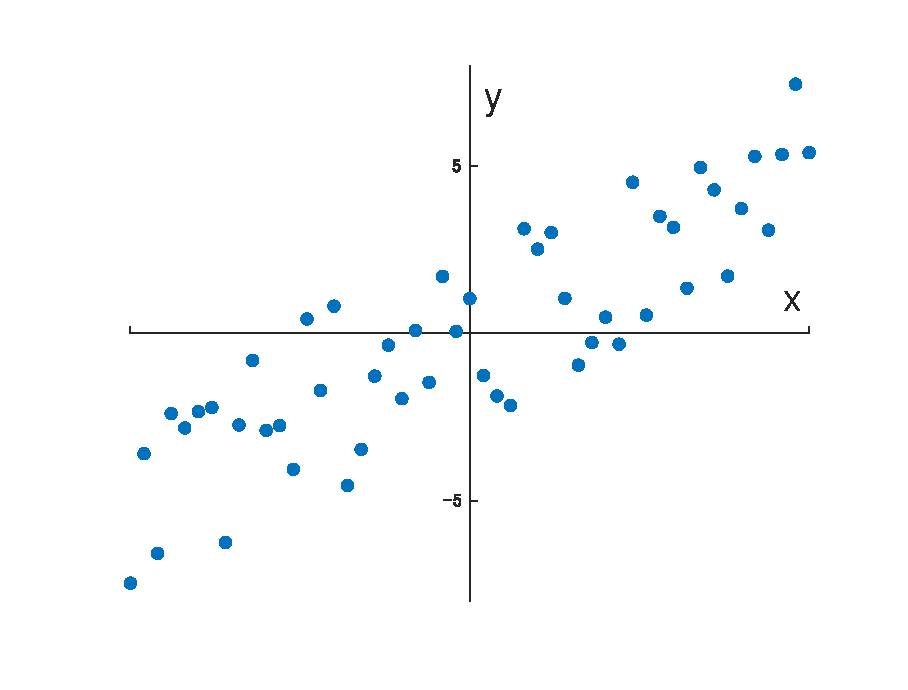
\includegraphics[width=10cm]{../figures/covar.eps}
  \caption{適当な散布図. どの象限に点が多いかで共分散の値が決まる}
\end{figure}

この2つを合わせる事で, 共分散は次のような性質を持ちます.\\
\\
 共分散は$S_xy$, 変数xと変数yの相関が強い程絶対値が大きくなり, その符号は相関の正負に一致する.
\\
式は以下です.\\
\begin{eqnarray}
\label{eq:covar}
S_{xy} = \frac{\sum_{i=1}^{n} (x_i - \bar{x})(y_i - \bar{y})}{n}
\end{eqnarray}

\begin{lstlisting}[caption=共分散のコード,label=sc:scatter keepspaces=true,]
x = [0:0.1:10]+ rand(1,101)
y = [0:0.1:10]

Sxy = (sum((x - mean(x)).*(y - mean(y))))/length(x)
cov(x,y)  // 関数を使うとこう(共分散行列)
\end{lstlisting}
共分散は,式(\ref{eq:covar})にもあるように$S_{xy}$などに求められるものです.2つの行列の場合,この組み合わせで4つ共分散が計算される事になります.つまり$S_{xy}, S_{xx}, S_{yy}, S_{yx}$です.これらを並べたものが共分散行列と言います.関数covはこれを求めるものです.\\
いうまでもなく,$S_{xx} = var(x)$です.図(\ref{im:co-var})の共分散行列を求めると,以下の結果が出ます.高いですね.

\begin{eqnarray}
\begin{matrix}
  1.0000 & 0.8555\\
  0.8555 & 1.0000\\
\end{matrix}
\end{eqnarray}

\subsection{相関係数}
ただ, 共分散は分散と違い, かけている変数の単位が違うため, 数字自体に意味はない事に注意が必要です. 例えばmmとmgで算出したときと, kmとkgで算出したときとでは同じデータなのに共分散の値が大きく変わってしまいますし, 単純に平方根を取ったところで違う単位系の積になってるので読み取れる情報がありません.\\
\\
 そこで, 共分散版の標準偏差的なものを定義してあげます. それが相関係数です.\\

\begin{eqnarray}
\label{eq:correlation}
r_{xy} = \frac{S_{xy}}{S_x S_y} = \frac{\frac{\sum_{i=1}^{n} (x_i - \bar{x})(y_i - \bar{y})}{n}}{\sqrt{\frac{\sum_{i=1}^{n} (x_i - \bar{x})^2}{n}} \sqrt{\frac{\sum_{i=1}^{n} (y_i - \bar{y})^2}{n}}}
\end{eqnarray}

\begin{lstlisting}[caption=共分散行列,label=sc:co-var]
x = [0:0.1:10]+ rand(1,101)
y = [0:0.1:10]

// ひ,ひぇぇ...
cov(x,y) / (std(x) * std(y)) // 
// つまり...
((sum((x - mean(x)).*(y - mean(y))))/length(x)) / (sqrt(sum((x - mean(x)).^2)/length(x)) * sqrt(sum((y - mean(y)).^2)/length(y)))

// 関数を使うとこう.相関係数行列
corrcoef(x,y)
\end{lstlisting}

分子が共分散になっているので, 分母にはそれぞれの標準偏差を入れているのですね. これにより相関係数はその単位に関係ない評価が出来るようになります. 当然, 共分散が標準偏差同士をかけたやつよりも上回る事はないので, 相関係数は -1から1の間の値を取ります.\\
 相関係数の値が-1に近い程負の相関が強く, 1に近い程正の相関が強いわけですね!!!便利です!!\\
 コードではやはり,corrcoefで相関係数行列を求めています.相関係数行列は全変数の組み合わせを$n \times n$行列ではきだすものです.対角成分は自分自身との相関なので1で,上半分と下半分は同じ変数の組み合わせなので対称になっています.よって上か下半分の三角形だけ見ればよいです.

\subsection{自己相関}
相関係数の亜種みたいなやつです.脳波のような時系列データ(データ$x_i$が時間$t_i$に対応して得らえれているデータ)は,ある時間の値が異なる時間の値に依存して変動するような事が考えられます.たとえば周期性なんかはまさにそうですよね.滑らかに変化するという事は,前の時間の値に依存しているとも言えるわけです.ということで,自分自身の異時点間での相関関係を見たくなるわけで,それが自己相関係数です.\\

 まずはデータを1時点ずらした信号との相関を考えます.すると

\begin{eqnarray}
\label{eq:self-corr0}
r = \frac{\frac{\sum_{i=1}^{n-1} (x_i-\bar x)(x_{i+1} - \bar x)}{n-1}}{\frac{\sum_{i=1}^n (x_i - \bar x)^2 /n}{n}}
\end{eqnarray}

という式に表せます.分子は$x_i, x_{i+1}$と,1ポイントずらした変数の組なので,組み合わせ(?)は$n-1$組になります.なのでそれらを使って共分散のようなものを計算します.この分子を特に自己共分散と呼びます.\\
 分母は普通の相関係数とは若干異なりますね.相関係数の場合は式(\ref{eq:correlation})にあるように分母は変数それぞれの標準偏差の積で正規化していました.しかしここでは,変数$x_i, x_{i+1}$はどちらも実質同じ集合なので,標準偏差も同じだと考えれば納得できるかと思います.同じ標準偏差をかけてるのだから,ただの分散ですよね.

まとめると自己相関係数とは,自己共分散を分散で割ったものとなります.式(\ref{eq:self-corr0})は時間のずれを1ポイントに指定していますが,別に制約はありません.ただ一般的には,時間のずれが大きくなるにつれて影響も小さくなりますよね.(例外はあります.周期をもってたりとか.)

てことで一般化するとこうなります.

\begin{eqnarray}
\label{eq:self-corr}
r = \frac{\frac{\sum_{i=1}^{n-h} (x_i-\bar x)(x_{i+h} - \bar x)}{n-h}}{\frac{\sum_{i=1}^n (x_i - \bar x)^2 /n}{n}}
\end{eqnarray}

ともかく,自己相関の値は負になる場合は次のタイミングには傾向が反転し,正になる場合には傾向が持続するような,そんな時系列データだよねということができます.無論,0に近い程自己相関は低いことになります.\\





\end{document}